\section{Method}
The method is summarized in figure~\ref{fig:workflow}. It consists of three main phases:
\begin{enumerate*}[(i)]
	\item feature extraction,
	\item classification, and
	\item delineation of linear elements.
\end{enumerate*}
%\bigskip
\begin{figure}[!b]
	\centering
	\begin{tikzpicture}[node distance=0.70cm, scale=0.7, every node/.style={transform shape}]
	
	\node (in1) [io] {Raw Point Cloud};
	
	\node (param) [title, below=of in1] {Feature extraction};
	\node (pro1) [process, below left=2.5cm and -1.6cm=of param, fill=darkorange!20] {Compute nearest neighbours};
	\node (pro2) [process, below=of pro1, fill=darkorange!20] {Compute neighbourhood features};
	
	\begin{scope}[on background layer]
	\node (fit1) [fit=(param)(pro1)(pro2), inner sep=4pt, transform shape=false, draw=black!80, fill=darkorange, fill opacity=0.5] {};
	\end{scope}
	
	\node (out1) [io, above right=-0.55cm and 4.5cm=of fit1] {Point Cloud Features};
	\node (in2) [io, right=of out1] {Manually Classified Point Cloud};
	
	\node (class) [title, below right=1.5cm and 5.7cm=of out1] {Classification};
	\node (pro4) [process, below left=2.5cm and -6.6cm=of class, fill=lightblue!20] {Remove irrelevant points};
	\node (pro5) [process, below=of pro4, fill=lightblue!20] {Create random forest classifier using manually classified point cloud};
	\node (pro6) [process, below=of pro5, fill=lightblue!20] {Assess performance using cross validation};
	\node (pro7) [process, above right=-3.67cm and 7.5cm=of pro6, fill=lightblue!20] {Classify unknown points};
	\node (pro8) [process, below=of pro7, fill=lightblue!20] {Compute cylindrical neighbourhoods of vegetation points};
	\node (pro9) [process, below=of pro8, fill=lightblue!20] {Seperate trees from low vegetation using height difference};
	
	\begin{scope}[on background layer]
	\node (fit2) [fit=(class)(pro4)(pro5)(pro6)(pro7)(pro8)(pro9), inner sep=4pt, transform shape=false, draw=black!80, fill=lightblue, fill opacity=0.5] {};
	\end{scope}
	
	\node (out2) [io, above right= -0.55cm and 13.5cm=of fit2] {Classified Point Cloud};
	
	\node (lin) [title, below=of out2] {Linear Elements};
	\node (pro10) [process, below left=2.5cm and -15.6cm=of lin, fill=turquoise!20] {Convert to 2D and downsample};
	\node (pro11) [process, below=of pro10, fill=turquoise!20] {Grow regions based on rectangularity};
	\node (pro12) [process, below=of pro11, fill=turquoise!20] {Merge directionally aligned regions};
	\node (pro13) [process, below=of pro12, fill=turquoise!20] {Assess the elongatedness of the regions};
	
	\begin{scope}[on background layer]
	\node (fit3) [fit=(lin)(pro10)(pro11)(pro12)(pro13), inner sep=4pt, transform shape=false, draw=black!80, fill=turquoise, fill opacity=0.5] {};
	\end{scope}
	
	\node (out3) [io, below=of fit3] {Linear vegetation elements};
	
	\draw [arrow] (in1) -- (fit1);
	\draw [arrow] (fit1) -| +(2.6,0) |- (out1.west);
	\draw [arrow] (out1.south) |- +(0,-0.45) -| (fit2.north); %(out1.south|-fit2.north);
	\draw [arrow] (fit2) -| +(4.5,0) |- (out2.west);
	\draw [arrow] (out2) -- (fit3);
	\draw [arrow] (in2.south) |- +(0,-0.195) -| (fit2.north); %(in2.south|-fit2.north);
	
	\draw [arrow] (pro1) -- (pro2);
	
	\draw [arrow] (pro4) -- (pro5);
	\draw [arrow] (pro5) -- (pro6);
	\draw [arrow] (pro5) -| +(2,0) |- (pro7);
	\draw [arrow] (pro7) -- (pro8);
	\draw [arrow] (pro8) -- (pro9);
	
	\draw [arrow] (pro10) -- (pro11);
	\draw [arrow] (pro11) -- (pro12);
	\draw [arrow] (pro12) -- (pro13);
	
	\draw [arrow] (fit3) -- (out3);
	
	\end{tikzpicture}
	\caption{Overview of the method in a work flow diagram.}
	\label{fig:workflow}
\end{figure}

\subsection{Feature extraction}
A point cloud \(\mathcal{P}\) is a set of points \(\{p_{1}, p_{2}, \dots, p_{n}\}\) \(\in \mathbb{R}^3\). Each point \(p_{i}\) consists of the X, Y and Z coordinates of the point and additional information on the intensity (\(I\)) of the return signal, the return number, and the number of returns (\(R_{t}\)) at \(p_{i}\) is known (figure~\ref{fig:LiDAR}).
A normalized return number (\(R_{n}\)) was calculated by dividing the return number by the number of returns~\citep{guo2011relevance}.

For each point \(p_{i}\) a neighbourhood set \(\mathcal{N}_{i}\) of points \(\{q_{1}, q_{2}, \dots, q_{k}\}\) is defined, where \(q_{1} = p_{i}\). 
%This can be done in three ways:
%\begin{enumerate*}[(i)]
%	\item a \(k\)-nearest neighbours neighbourhood, where the first \(k\ (-1)\) nearest points to \(p_{i}\) are part of the neighbourhood,
%	\item a spherical neighbourhood, where all the points within a certain radius (\(r_{s}\)) of \(p_{i}\) belong to the neighbourhood, and
%	\item a cylindrical neighbourhood, which includes all points within a cylinder with infinite height and a certain radius (\(r_{c}\)) of \(p_{i}\).
%\end{enumerate*}
This neighbourhood was determined using a \(k\)-nearest neighbours method with a \(k\) of 50. This method was used instead of spherical neighbourhood of a certain radius, because it is harder to define a suitable radius which works for fluctuating point densities within and across datasets~\citep{weinmann2014semantic}.

To determine these neighbours a k-d tree data structure was constructed, which is a multidimensional binary search tree that can be used for efficient nearest neighbour searches~\citep{bentley1975kdtree}.

For each neighbourhood some basic geometric properties are computed \citep{weinmann2015semantic}:

{\setlength{\abovedisplayskip}{0pt}
\begin{flalign}
	\label{eq:deltaz}
	&\text{Height difference:}&&& \Delta_{Z_{i}} &= \max_{j:\mathcal{N}_{i}}(q_{Z_{j}}) - \min_{j:\mathcal{N}_{i}}(q_{Z_{j}}) &&&\\
	\label{eq:stdz}
	&\text{Height standard deviation:}&&& \sigma_{Z_{i}} &= \sqrt{\frac{1}{k} \sum_{j=1}^k (q_{Z_{j}} - \overline{q_{Z}})^2} &&&\\
	\label{eq:radius}
	&\text{Local radius:}&&& r_{l_{i}} &= \max_{j: \mathcal{N}_{i}}(|p_{i} - q_{j}|) &&&\\
	\label{eq:density}
	&\text{Local point density:}&&& D_{i} &= \frac{k}{\frac{4}{3} \pi r_{l_{i}}^3} &&&
\end{flalign}

Additionally the neighbourhood of a point can be used to characterize local surface features as first described by~\citet{hoppe1992surface}, and further developed by~\citet{pauly2002efficient}, who used the local structure tensor to estimate the surface normals (the vector perpendicular to the surface (\(\vec{N} = (N_{x}, N_{y}, N_{z})\))) and to define the surface variation (equation~\ref{eq:surfacevariation}). The structure tensor describes the directions of the neighbourhood of a point by determining the covariance matrix of the X, Y and Z coordinates of the points and computing the eigenvalues (\(\lambda_{1}, \lambda_{2}, \lambda_{3}\), where \(\lambda_{1} > \lambda_{2} > \lambda_{3}\)) and eigenvectors of this matrix. The magnitude of the eigenvalues of this covariance matrix describe the spread of points in the direction of the eigenvector. By ranking the eigenvectors based on the respective eigenvalues the spread in the three principle directions of a local point cloud can be quantified. This was expanded upon by~\citet{west2004context} to the following eight structure tensor features:

\begin{flalign}
\label{eq:linearity}
&\text{Linearity: }&&& L_{\lambda} &= \frac{\lambda_{1} - \lambda_{2}}{\lambda_{1}}&&&\\
\label{eq:planarity}
&\text{Planarity: }&&& P_{\lambda} &= \frac{\lambda_{2} - \lambda_{3}}{\lambda_{1}}&&&\\
\label{eq:sphericity}
&\text{Sphericity: }&&& S_{\lambda} &= \frac{\lambda_{3}}{\lambda_{1}}&&&\\
\label{eq:omnivariance}
&\text{Omnivariance: }&&& O_{\lambda} &= \sqrt[3]{\lambda_{1} \lambda_{2} \lambda_{3}}&&&\\
\label{eq:anisotropy}
&\text{Anisotropy: }&&& A_{\lambda} &= \frac{\lambda_{1} - \lambda_{3}}{\lambda_{1}}&&&\\
\label{eq:eigenentropy}
&\text{Eigenentropy: }&&& E_{\lambda} &= -\lambda_{1}\ln(\lambda_{1}) -\lambda_{2}\ln(\lambda_{2}) -\lambda_{3}\ln(\lambda_{3})&&&\\
\label{eq:sumofeigenvalues}
&\text{Sum of eigenvalues: }&&& \sum_{\lambda} &= \lambda_{1} + \lambda_{2} + \lambda_{3}&&&\\
\label{eq:surfacevariation}
&\text{Local surface variation: }&&& C_{\lambda} &= \frac{\lambda_{3}}{\lambda_{1} + \lambda_{2} + \lambda_{3}}&&&
\end{flalign}

To avoid using an unnecessarily large feature set the correlation between all the features was checked by calculating pearson coefficients. Of the pairs of two extremely correlated features (above 0.98), one was removed. This resulted in the removal of anisotropy, which is negatively correlated with sphericity, and eigenentropy, which is correlated with omnivariance.

Consequently the resulting feature set used for the classification was \(\{I, R_{t}, R_{n}, \Delta_{Z}, \sigma_{Z}, r_{l}, D, N_{z}, L_{\lambda}, P_{\lambda}, S_{\lambda}, O_{\lambda}, \sum_{\lambda}, C_{\lambda}\}\).

\subsection{Classification}
\label{sec:class}
Since the linear vegetation elements consist of either trees or low vegetation (shrubs and small trees) the point cloud needs to be classified into \textit{trees}, \textit{low vegetation}, and \textit{irrelevant} points. The difference between trees and low vegetation is ambiguous and is dependent on interpretation. In previous research this boundary has been set at varying height values, ranging from 1.5~\citep{bork2007integrating}, to 3.5~\citep{antonarakis2008object}, to 4~\citep{koukoulas2005spatial}, to 5 meters~\citep{khosravipour2014generating}. We set this boundary at 4m. The irrelevant points are returns of which the linearity does not need to be checked. This may include very low vegetation (herbs), bare ground, water, buildings, and other man made objects.

\subsubsection{Data trimming}
To speed up the classification first points were removed which were certain not relevant. This was done based on the planarity (equation~\ref{eq:planarity}) and sphericity (equation~\ref{eq:sphericity}) features discussed earlier. Since scanning vegetation (which is larger than herbs) always results in a locally very scattered point cloud, with points spread out throughout the 3D space, points with a locally planar neighbourhood can be removed. That is to say points with a high planarity value, \(P_{\lambda} > 0.7\), and a low sphericity value, \(S_{\lambda} < 0.05\), were removed. These values were manually selected in a conservative way to make sure every point removed was certainly not relevant, while still removing a large portion of points.
 
\subsubsection{Supervised classification}
The remaining point cloud was classified into \textit{vegetation} and \textit{irrelevant} using a random forest classifier. The random forest algorithm creates a collection of decision trees each based on a random subset of the training data~\citep{ho1998random}. These decision trees are computed by a Classification And Regression Tree (CART) algorithm, which creates splits that minimize a gini impurity index~\citep{breiman1984classification}. This impurity index is the probability a randomly picked sample would be misclassified, given it was randomly classified conform the distribution of classes. For each point, each tree in the forest determines a class, and the class which gets selected by the majority of the trees is chosen as the final classification~\citep{breiman2001random}.

Training and testing data was created by analysing the research area and manually segmenting areas of \textit{vegetation} and \textit{irrelevant}. This was done based on the point cloud and aerial photos~\citep{PDOK2015luchtfoto}. 

Because the point cloud is trimmed based on planarity/sphericity and it concerns an agricultural landscape it has become very imbalanced, having a lot more \textit{vegetation} than \textit{irrelevant} points, which was also very noticeable in the training and testing data. Imbalanced training data can lead to undesirable classification results~\citep{he2009learning}. Therefore a balanced random forest was used, where instead of the decision trees being made using bootstrap samples of the entire training dataset, a bootstrap sample was taken from only the minority class and a random sample was taken of the majority class based on the size of the minority class sample~\citep{Chen2004using}. Employing enough trees eventually all majority class data gets used, while still maintaining a balance between the two classes. The size of the majority sample compared to the minority sample can be adjusted to find the best balance.

The random forest parameters (i.e. maximum depth, maximum number of features, minimal samples per leaf, minimal samples per split) and the ratio between minority and majority samples were optimized using a cross validated grid search.

\subsubsection{Accuracy Assessment}

To assess the accuracy of the classification a confusion matrix was used. Such a matrix shows the predicted and the actual classes of the tested pixels/points. It gives an overview of the performance of the classification in that it identifies and quantifies the errors. Using this matrix a precision (user's accuracy), recall (producer's accuracy), and overall accuracy can be calculated~\citep{stehman1997selecting}, but these metrics are unable to provide a good picture of the performance of a classifier when the data is very imbalanced.

Instead, three metrics, which provide a useful indication of performance even when dealing with a very imbalanced dataset, were used~\citep{sun2009classification, lopez2013insight}. These are:
\begin{enumerate*}[(i)]
	\item the receiver operating characteristic (ROC) curve~\citep{bradley1997use},
	\item the Matthew's correlation coefficient (MCC)~\citep{matthews1975comparison}, and
	\item the geometric mean~\citep{kubat1998machine}.
\end{enumerate*}

To create a ROC-curve the true positive rate is plotted against the false positive rate at various decision thresholds. The area under a ROC-curve (AUC) is a measure for the performance of the classifier~\citep{bradley1997use}.

The MCC analyses the correlation between the observed and the predicted data and is defined as follows:

\begin{equation}
	\label{eq:MCC}
	{\text{MCC}}={\frac  {TP\times TN-FP\times FN}{{\sqrt  {(TP+FP)(TP+FN)(TN+FP)(TN+FN)}}}}
\end{equation}

where TP are the true positives, TN the true negatives, FP the false positives, and FN the false negatives. It often gives a more balanced evaluation of a classifier than the precision, recall and accuracy~\citep{baldi2000assessing} and it is an effective metric for unbalanced datasets~\citep{kohavi1995study}.

The geometric mean of the recall of both classes evaluates the balanced performance of the classifier for the two classes~\citep{kubat1998machine, sun2009classification}.

These scores were acquired by performing a 10-fold cross validation. This is done by splitting the data into 10 randomly mutually exclusive subsets and using a subset as testing data on a classifier trained on the remaining data~\citep{kohavi1995study}. This method is effective against overfitting and does not further reduce the training data (which a test and validation set would).

To assess which features are most influential when separating vegetation from non-vegetation a feature importance analysis was performed. This is done by summing the decreases in gini impurity due to a feature in all the trees divided by the total amount of trees~\citep{breiman2002manual}.

\subsubsection{Delineating trees and low vegetation}
To divide the vegetation class into \textit{tree} and \textit{low vegetation} for each point a cylindrical neighbourhood was determined, which includes all points within a cylinder with infinite height and a radius of 2 meters. Within this neighbourhood the height difference (equation~\ref{eq:deltaz}) was computed. As mentioned earlier, if this value exceeded 4 meters the point was classified as a \textit{tree} point, otherwise as a \textit{low vegetation} point.

\subsection{Delineating Linear Elements}
To delineate linear from non-linear vegetation elements the two classes were segmented into rectangular objects, since those can be assessed for linearity by their length and width. This is done by growing regions within the relevant points as long as the shape remains rectangular. 

\begin{figure}
	\centering
	\includegraphics[scale=0.40]{./img/downsample}
	\caption{An example showing the tree points before and after downsampling.}
	\label{fig:downsample}
\end{figure}
Since the linearity of an object is solely determined by the 2D spatial distribution of points, the point cloud was converted to 2D by removing the Z-coordinate from all the points. To speed up the computation the 2D point cloud was spatially downsampled to 1 meter distance between all points for low vegetation and 2 meter for trees (figure~\ref{fig:downsample}). Low vegetation objects are often smaller than trees and consequently require more points for an accurate delineation. This leads to a slightly less precise delineation, but results in a substantially decreased computation time.

\subsubsection{Rectangularity}
\begin{figure}
	\centering
	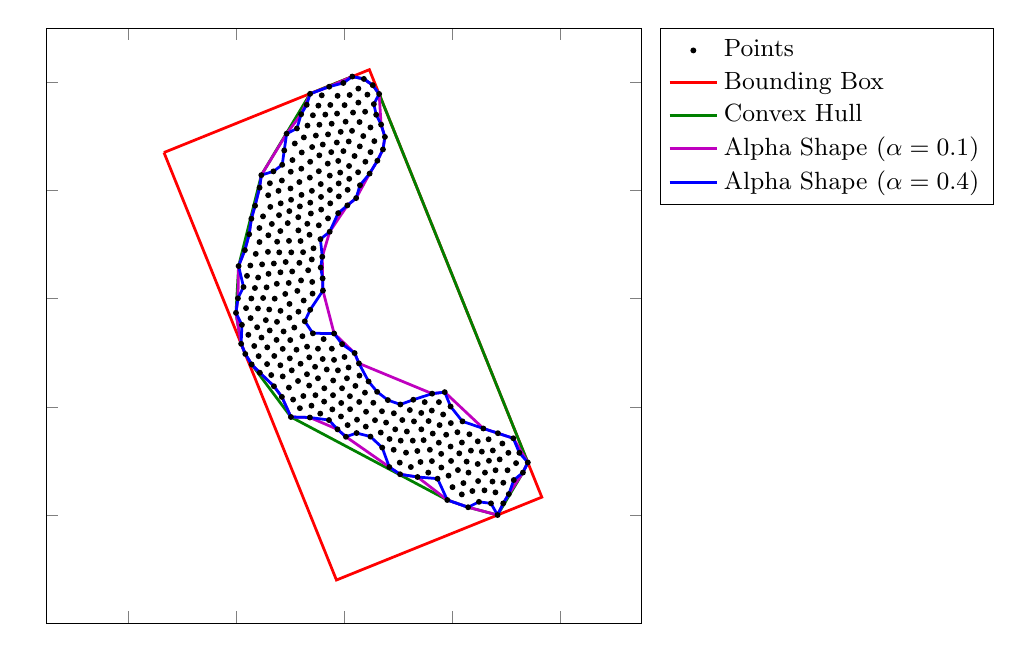
\begin{tikzpicture}%[scale=1.1]

\definecolor{color0}{rgb}{0.75,0,0.75}

\begin{axis}[
%scale only axis=true,
width=260,
height=260,
xmin=-35, xmax=75,
ymin=-20, ymax=90,
yticklabels={,,},
xticklabels={,,},
%axis on top,
%tick pos=both,
legend entries={{Points},{Bounding Box},{Convex Hull},{Alpha Shape
		(\(\alpha=0.1\))},{Alpha Shape
		(\(\alpha=0.4\))}},
legend cell align={left},
legend pos=outer north east,
legend style={font=\small}
]
\addplot [only marks, draw=black, fill=black, mark size=0.85, colormap={mymap}{[1pt]
  rgb(0pt)=(0,0,0.5);
rgb(22pt)=(0,0,1);
rgb(25pt)=(0,0,1);
rgb(68pt)=(0,0.86,1);
rgb(70pt)=(0,0.9,0.967741935483871);
rgb(75pt)=(0.0806451612903226,1,0.887096774193548);
rgb(128pt)=(0.935483870967742,1,0.0322580645161291);
rgb(130pt)=(0.967741935483871,0.962962962962963,0);
rgb(132pt)=(1,0.925925925925926,0);
rgb(178pt)=(1,0.0740740740740741,0);
rgb(182pt)=(0.909090909090909,0,0);
rgb(200pt)=(0.5,0,0)
}]
table{%
x                      y
+5.395319999998901e+01 +9.718799999973271e+00
+5.304689999998664e+01 +7.843799999973271e+00
+5.239069999998901e+01 +1.150000000000000e+01
+5.178129999997327e+01 +9.593799999973271e+00
+5.135939999998664e+01 +6.468799999973271e+00
+5.043750000000000e+01 +3.875000000000000e+00
+5.126569999998901e+01 +1.418750000000000e+01
+5.020319999998901e+01 +8.281299999973271e+00
+4.940629999997327e+01 +2.156299999973271e+00
+5.035939999998664e+01 +1.150000000000000e+01
+4.942189999998664e+01 +5.968799999973271e+00
+4.835939999998664e+01 +0.000000000000000e+00
+4.925000000000000e+01 +1.321879999997327e+01
+4.875000000000000e+01 +1.028129999997327e+01
+4.796879999997327e+01 +4.187500000000000e+00
+4.798439999998664e+01 +8.281299999973271e+00
+4.714069999998901e+01 +2.156299999973271e+00
+4.742189999998664e+01 +6.187500000000000e+00
+4.842189999998664e+01 +1.512500000000000e+01
+4.748439999998664e+01 +1.193750000000000e+01
+4.676569999998901e+01 +1.003129999997327e+01
+4.593750000000000e+01 +4.562500000000000e+00
+4.603129999997327e+01 +7.843799999973271e+00
+4.670319999998901e+01 +1.400000000000000e+01
+4.492189999998664e+01 +2.437500000000000e+00
+4.545319999998901e+01 +1.171879999997327e+01
+4.476569999998901e+01 +6.281299999973271e+00
+4.573439999998664e+01 +1.600000000000000e+01
+4.468750000000000e+01 +9.437500000000000e+00
+4.370319999998901e+01 +4.437500000000000e+00
+4.470319999998901e+01 +1.362500000000000e+01
+4.292189999998664e+01 +1.437500000000000e+00
+4.298439999998664e+01 +7.843799999973271e+00
+4.343750000000000e+01 +1.190629999997327e+01
+4.264069999998901e+01 +9.875000000000000e+00
+4.204689999998664e+01 +5.906299999973271e+00
+4.175000000000000e+01 +3.812500000000000e+00
+4.315629999997327e+01 +1.493750000000000e+01
+4.176569999998901e+01 +1.340629999997327e+01
+4.103129999997327e+01 +8.312500000000000e+00
+4.128129999997327e+01 +1.140629999997327e+01
+4.187500000000000e+01 +1.731250000000000e+01
+4.003129999997327e+01 +5.156299999973271e+00
+4.093750000000000e+01 +1.531250000000000e+01
+3.906250000000000e+01 +2.781299999973271e+00
+3.976569999998901e+01 +1.000000000000000e+01
+3.929689999998664e+01 +7.281299999973271e+00
+3.967189999998664e+01 +1.265629999997327e+01
+3.971879999997327e+01 +1.700000000000000e+01
+3.967189999998664e+01 +2.006250000000000e+01
+3.885939999998664e+01 +1.484379999997327e+01
+3.796879999997327e+01 +8.781299999973271e+00
+3.793750000000000e+01 +1.131250000000000e+01
+3.726569999998901e+01 +6.718799999973271e+00
+3.829689999998664e+01 +1.859379999997327e+01
+3.750000000000000e+01 +1.337500000000000e+01
+3.859379999997327e+01 +2.271879999997327e+01
+3.764069999998901e+01 +1.662500000000000e+01
+3.621879999997327e+01 +9.968799999973271e+00
+3.751569999998901e+01 +2.087500000000000e+01
+3.554689999998664e+01 +7.843799999973271e+00
+3.637500000000000e+01 +1.506250000000000e+01
+3.584379999997327e+01 +1.206250000000000e+01
+3.620319999998901e+01 +1.931250000000000e+01
+3.626569999998901e+01 +2.243750000000000e+01
+3.560939999998664e+01 +1.737500000000000e+01
+3.468750000000000e+01 +1.384379999997327e+01
+3.410939999998664e+01 +9.812500000000000e+00
+3.356250000000000e+01 +7.031299999973271e+00
+3.489069999998901e+01 +2.087500000000000e+01
+3.426569999998901e+01 +1.584379999997327e+01
+3.353129999997327e+01 +1.184379999997327e+01
+3.425000000000000e+01 +1.887500000000000e+01
+3.232819999998901e+01 +8.875000000000000e+00
+3.268750000000000e+01 +1.375000000000000e+01
+3.290629999997327e+01 +1.731250000000000e+01
+3.278129999997327e+01 +2.131250000000000e+01
+3.143750000000000e+01 +1.153129999997327e+01
+3.214069999998901e+01 +1.940629999997327e+01
+3.159379999997327e+01 +1.543750000000000e+01
+3.034379999997327e+01 +7.531299999973271e+00
+3.028129999997327e+01 +9.687500000000000e+00
+3.045319999998901e+01 +1.375000000000000e+01
+3.075000000000000e+01 +1.756250000000000e+01
+3.039069999998901e+01 +2.043750000000000e+01
+2.915629999997327e+01 +1.206250000000000e+01
+2.943750000000000e+01 +1.584379999997327e+01
+2.834379999997327e+01 +8.875000000000000e+00
+2.918750000000000e+01 +1.881250000000000e+01
+2.839069999998901e+01 +1.406250000000000e+01
+2.775000000000000e+01 +1.709379999997327e+01
+2.703129999997327e+01 +1.246879999997327e+01
+2.807819999998901e+01 +2.125000000000000e+01
+2.676569999998901e+01 +1.525000000000000e+01
+2.698439999998664e+01 +1.918750000000000e+01
+2.570319999998901e+01 +1.753129999997327e+01
+2.609379999997327e+01 +2.278129999997327e+01
+2.485939999998664e+01 +1.450000000000000e+01
+2.539069999998901e+01 +2.075000000000000e+01
+2.400000000000000e+01 +1.634379999997327e+01
+2.404689999998664e+01 +1.909379999997327e+01
+2.451569999998901e+01 +2.468750000000000e+01
+2.384379999997327e+01 +2.262500000000000e+01
+2.229689999998664e+01 +1.515629999997327e+01
+2.278129999997327e+01 +2.090629999997327e+01
+2.237500000000000e+01 +1.762500000000000e+01
+2.282819999998901e+01 +2.578129999997327e+01
+2.273439999998664e+01 +2.803129999997327e+01
+2.207819999998901e+01 +2.387500000000000e+01
+2.109379999997327e+01 +1.956250000000000e+01
+2.064069999998901e+01 +1.662500000000000e+01
+2.032819999998901e+01 +1.446879999997327e+01
+2.106250000000000e+01 +2.196879999997327e+01
+2.193750000000000e+01 +2.993750000000000e+01
+2.081250000000000e+01 +2.728129999997327e+01
+2.051569999998901e+01 +2.528129999997327e+01
+1.940629999997327e+01 +1.821879999997327e+01
+1.945319999998901e+01 +2.071879999997327e+01
+1.876569999998901e+01 +1.584379999997327e+01
+1.960939999998664e+01 +2.343750000000000e+01
+2.006250000000000e+01 +2.921879999997327e+01
+1.962500000000000e+01 +3.159379999997327e+01
+1.884379999997327e+01 +2.675000000000000e+01
+1.781250000000000e+01 +1.953129999997327e+01
+1.793750000000000e+01 +2.215629999997327e+01
+1.718750000000000e+01 +1.756250000000000e+01
+1.796879999997327e+01 +2.487500000000000e+01
+1.812500000000000e+01 +2.868750000000000e+01
+1.814069999998901e+01 +3.356250000000000e+01
+1.771879999997327e+01 +3.075000000000000e+01
+1.629689999998664e+01 +2.096879999997327e+01
+1.678129999997327e+01 +2.690629999997327e+01
+1.632819999998901e+01 +2.343750000000000e+01
+1.557819999998901e+01 +1.875000000000000e+01
+1.603129999997327e+01 +2.884379999997327e+01
+1.620319999998901e+01 +3.253129999997327e+01
+1.515629999997327e+01 +2.528129999997327e+01
+1.468750000000000e+01 +2.215629999997327e+01
+1.395319999998901e+01 +2.021879999997327e+01
+1.365629999997327e+01 +1.803129999997327e+01
+1.515629999997327e+01 +3.075000000000000e+01
+1.462500000000000e+01 +2.740629999997327e+01
+1.607819999998901e+01 +4.150000000000000e+01
+1.353129999997327e+01 +2.393750000000000e+01
+1.601569999998901e+01 +4.375000000000000e+01
+1.421879999997327e+01 +3.359379999997327e+01
+1.354689999998664e+01 +2.915629999997327e+01
+1.312500000000000e+01 +2.603129999997327e+01
+1.245319999998901e+01 +2.200000000000000e+01
+1.595319999998901e+01 +4.775000000000000e+01
+1.565629999997327e+01 +4.575000000000000e+01
+1.181250000000000e+01 +1.975000000000000e+01
+1.314069999998901e+01 +3.112500000000000e+01
+1.415629999997327e+01 +4.093750000000000e+01
+1.371879999997327e+01 +3.793750000000000e+01
+1.409379999997327e+01 +4.309379999997327e+01
+1.193750000000000e+01 +2.796879999997327e+01
+1.146879999997327e+01 +2.478129999997327e+01
+1.271879999997327e+01 +3.581250000000000e+01
+1.228129999997327e+01 +3.306250000000000e+01
+1.015629999997327e+01 +1.812500000000000e+01
+1.056250000000000e+01 +2.134379999997327e+01
+1.401569999998901e+01 +4.725000000000000e+01
+1.334379999997327e+01 +4.525000000000000e+01
+1.251569999998901e+01 +3.965629999997327e+01
+1.118750000000000e+01 +3.056250000000000e+01
+1.031250000000000e+01 +2.675000000000000e+01
+9.781299999973271e+00 +2.356250000000000e+01
+1.154689999998664e+01 +3.759379999997327e+01
+1.203129999997327e+01 +4.337500000000000e+01
+1.078129999997327e+01 +3.465629999997327e+01
+9.953199999989010e+00 +2.896879999997327e+01
+1.240629999997327e+01 +4.859379999997327e+01
+1.134379999997327e+01 +4.143750000000000e+01
+1.003129999997327e+01 +3.234379999997327e+01
+8.484399999986636e+00 +2.184379999997327e+01
+1.171879999997327e+01 +4.662500000000000e+01
+8.640699999989010e+00 +2.562500000000000e+01
+9.875000000000000e+00 +3.646879999997327e+01
+9.890699999989010e+00 +3.903129999997327e+01
+8.640699999989010e+00 +3.071879999997327e+01
+8.203199999989010e+00 +2.768750000000000e+01
+1.039069999998901e+01 +4.503129999997327e+01
+8.796899999986636e+00 +3.393750000000000e+01
+9.750000000000000e+00 +4.290629999997327e+01
+7.015699999989010e+00 +2.381250000000000e+01
+1.021879999997327e+01 +4.856250000000000e+01
+9.109399999986636e+00 +4.087500000000000e+01
+8.234399999986636e+00 +3.775000000000000e+01
+7.500000000000000e+00 +3.237500000000000e+01
+7.078199999989010e+00 +2.940629999997327e+01
+6.515699999989010e+00 +2.587500000000000e+01
+9.187500000000000e+00 +4.678129999997327e+01
+7.578199999989010e+00 +3.571879999997327e+01
+8.218799999973271e+00 +4.487500000000000e+01
+5.750000000000000e+00 +2.790629999997327e+01
+7.546899999986636e+00 +4.275000000000000e+01
+7.156299999973271e+00 +4.000000000000000e+01
+6.234399999986636e+00 +3.412500000000000e+01
+5.781299999973271e+00 +3.100000000000000e+01
+8.000000000000000e+00 +4.856250000000000e+01
+6.140699999989010e+00 +3.800000000000000e+01
+4.406299999973271e+00 +2.631250000000000e+01
+7.000000000000000e+00 +4.650000000000000e+01
+5.515699999989010e+00 +3.603129999997327e+01
+4.718799999973271e+00 +3.281250000000000e+01
+4.187500000000000e+00 +2.937500000000000e+01
+6.015699999989010e+00 +4.459379999997327e+01
+5.656299999973271e+00 +4.209379999997327e+01
+5.015699999989010e+00 +4.012500000000000e+01
+5.906299999973271e+00 +4.865629999997327e+01
+3.906299999973271e+00 +3.471879999997327e+01
+3.375000000000000e+00 +3.125000000000000e+01
+2.890699999989010e+00 +2.784379999997327e+01
+4.062500000000000e+00 +3.818750000000000e+01
+4.828199999989010e+00 +4.634379999997327e+01
+4.093799999973271e+00 +4.390629999997327e+01
+3.500000000000000e+00 +4.196879999997327e+01
+2.703199999989010e+00 +3.640629999997327e+01
+2.281299999973271e+00 +3.331250000000000e+01
+1.718799999973271e+00 +2.978129999997327e+01
+2.843799999973271e+00 +4.003129999997327e+01
+3.656299999973271e+00 +4.828129999997327e+01
+1.859399999986636e+00 +3.825000000000000e+01
+9.531999999890104e-01 +3.165629999997327e+01
+2.656299999973271e+00 +4.612500000000000e+01
+1.093799999973271e+00 +3.515629999997327e+01
+2.031299999973271e+00 +4.421879999997327e+01
+1.390699999989010e+00 +4.215629999997327e+01
+1.640699999989010e+00 +4.896879999997327e+01
+3.593999999866355e-01 +4.006250000000000e+01
+0.000000000000000e+00 +3.737500000000000e+01
+4.843999999866355e-01 +4.603129999997327e+01
+2.753129999997327e+01 +6.990629999997327e+01
+2.717189999998664e+01 +6.759379999997327e+01
+2.614069999998901e+01 +6.550000000000000e+01
+2.682819999998901e+01 +7.218750000000000e+01
+2.557819999998901e+01 +6.912500000000000e+01
+2.470319999998901e+01 +6.312500000000000e+01
+2.646879999997327e+01 +7.784379999997327e+01
+2.592189999998664e+01 +7.400000000000000e+01
+2.487500000000000e+01 +6.709379999997327e+01
+2.548439999998664e+01 +7.596879999997327e+01
+2.485939999998664e+01 +7.165629999997327e+01
+2.392189999998664e+01 +6.531250000000000e+01
+2.292189999998664e+01 +6.096879999997327e+01
+2.528129999997327e+01 +7.946879999997327e+01
+2.221879999997327e+01 +5.859379999997327e+01
+2.353129999997327e+01 +7.006250000000000e+01
+2.257819999998901e+01 +6.337500000000000e+01
+2.429689999998664e+01 +7.771879999997327e+01
+2.387500000000000e+01 +7.456250000000000e+01
+2.289069999998901e+01 +6.815629999997327e+01
+2.284379999997327e+01 +7.265629999997327e+01
+2.192189999998664e+01 +6.637500000000000e+01
+2.059379999997327e+01 +5.725000000000000e+01
+2.364069999998901e+01 +8.062500000000000e+01
+2.093750000000000e+01 +6.215629999997327e+01
+2.064069999998901e+01 +6.012500000000000e+01
+2.262500000000000e+01 +7.625000000000000e+01
+2.090629999997327e+01 +6.453129999997327e+01
+2.262500000000000e+01 +7.884379999997327e+01
+2.145319999998901e+01 +7.103129999997327e+01
+2.164069999998901e+01 +7.440629999997327e+01
+2.084379999997327e+01 +6.906250000000000e+01
+1.889069999998901e+01 +5.581250000000000e+01
+1.901569999998901e+01 +5.890629999997327e+01
+1.985939999998664e+01 +6.728129999997327e+01
+1.926569999998901e+01 +6.331250000000000e+01
+1.898439999998664e+01 +6.131250000000000e+01
+2.150000000000000e+01 +8.106250000000000e+01
+2.101569999998901e+01 +7.765629999997327e+01
+2.026569999998901e+01 +7.271879999997327e+01
+1.732819999998901e+01 +5.237500000000000e+01
+1.890629999997327e+01 +6.546879999997327e+01
+2.007819999998901e+01 +7.578129999997327e+01
+1.935939999998664e+01 +7.084379999997327e+01
+1.742189999998664e+01 +5.762500000000000e+01
+1.701569999998901e+01 +5.484379999997327e+01
+1.864069999998901e+01 +6.887500000000000e+01
+1.735939999998664e+01 +6.009379999997327e+01
+1.984379999997327e+01 +7.987500000000000e+01
+1.734379999997327e+01 +6.275000000000000e+01
+1.560939999998664e+01 +5.100000000000000e+01
+1.868750000000000e+01 +7.421879999997327e+01
+1.760939999998664e+01 +6.709379999997327e+01
+1.878129999997327e+01 +7.750000000000000e+01
+1.696879999997327e+01 +6.496879999997327e+01
+1.575000000000000e+01 +5.646879999997327e+01
+1.531250000000000e+01 +5.356250000000000e+01
+1.768750000000000e+01 +7.234379999997327e+01
+1.571879999997327e+01 +5.881250000000000e+01
+1.432819999998901e+01 +4.931250000000000e+01
+1.701569999998901e+01 +7.037500000000000e+01
+1.567189999998664e+01 +6.118750000000000e+01
+1.743750000000000e+01 +7.581250000000000e+01
+1.604689999998664e+01 +6.850000000000000e+01
+1.531250000000000e+01 +6.356250000000000e+01
+1.359379999997327e+01 +5.181250000000000e+01
+1.723439999998664e+01 +7.918750000000000e+01
+1.651569999998901e+01 +7.403129999997327e+01
+1.540629999997327e+01 +6.650000000000000e+01
+1.384379999997327e+01 +5.575000000000000e+01
+1.403129999997327e+01 +5.993750000000000e+01
+1.373439999998664e+01 +5.775000000000000e+01
+1.318750000000000e+01 +5.384379999997327e+01
+1.542189999998664e+01 +7.215629999997327e+01
+1.585939999998664e+01 +7.759379999997327e+01
+1.476569999998901e+01 +7.015629999997327e+01
+1.365629999997327e+01 +6.237500000000000e+01
+1.193750000000000e+01 +5.065629999997327e+01
+1.523439999998664e+01 +7.568750000000000e+01
+1.407819999998901e+01 +6.803129999997327e+01
+1.371879999997327e+01 +6.531250000000000e+01
+1.153129999997327e+01 +5.262500000000000e+01
+1.421879999997327e+01 +7.390629999997327e+01
+1.210939999998664e+01 +5.918750000000000e+01
+1.181250000000000e+01 +5.706250000000000e+01
+1.151569999998901e+01 +5.506250000000000e+01
+1.321879999997327e+01 +7.200000000000000e+01
+1.207819999998901e+01 +6.403129999997327e+01
+1.171879999997327e+01 +6.156250000000000e+01
+1.370319999998901e+01 +7.787500000000000e+01
+1.254689999998664e+01 +6.981250000000000e+01
+1.215629999997327e+01 +6.703129999997327e+01
+9.796899999986636e+00 +5.068750000000000e+01
+1.307819999998901e+01 +7.584379999997327e+01
+1.018750000000000e+01 +5.828129999997327e+01
+9.859399999986636e+00 +5.618750000000000e+01
+9.562500000000000e+00 +5.396879999997327e+01
+1.204689999998664e+01 +7.409379999997327e+01
+1.007819999998901e+01 +6.037500000000000e+01
+1.126569999998901e+01 +7.146879999997327e+01
+1.087500000000000e+01 +6.868750000000000e+01
+1.043750000000000e+01 +6.562500000000000e+01
+1.012500000000000e+01 +6.346879999997327e+01
+8.203199999989010e+00 +5.250000000000000e+01
+7.609399999986636e+00 +5.053129999997327e+01
+8.265699999989010e+00 +5.762500000000000e+01
+7.953199999989010e+00 +5.543750000000000e+01
+8.484399999986636e+00 +6.184379999997327e+01
+9.359399999986636e+00 +7.050000000000000e+01
+8.921899999986636e+00 +6.740629999997327e+01
+8.546899999986636e+00 +6.475000000000000e+01
+7.859399999986636e+00 +5.993750000000000e+01
+6.625000000000000e+00 +5.381250000000000e+01
+5.984399999986636e+00 +5.171879999997327e+01
+6.343799999973271e+00 +5.696879999997327e+01
+6.921899999986636e+00 +6.353129999997327e+01
+6.265699999989010e+00 +6.134379999997327e+01
+5.953199999989010e+00 +5.912500000000000e+01
+5.000000000000000e+00 +5.521879999997327e+01
+4.343799999973271e+00 +5.046879999997327e+01
+4.328199999989010e+00 +5.306250000000000e+01
+4.687500000000000e+00 +6.284379999997327e+01
+4.359399999986636e+00 +6.053129999997327e+01
+3.531299999973271e+00 +5.718750000000000e+01
+2.843799999973271e+00 +5.478129999997327e+01
+2.437500000000000e+00 +5.190629999997327e+01
};
\addplot [red, line width=0.35mm]
table {%
-13.312961844268 67.0175331227428
24.6564822832176 82.3359535290263
56.542278314707 3.30130643307495
18.5728341872214 -12.0171139732086
-13.312961844268 67.0175331227428
};
\addplot [green!50.0!black, line width=0.35mm]
table {%
48.3593999999866 0
42.9218999999866 1.4375
39.0625 2.78129999997327
10.1562999999733 18.125
2.89069999998901 27.8437999999733
1.71879999997327 29.7812999999733
0.95319999998901 31.6562999999733
0 37.375
0.484399999986636 46.0312999999733
4.6875 62.8437999999733
13.703199999989 77.875
21.5 81.0625
23.640699999989 80.625
25.2812999999733 79.4687999999733
26.4687999999733 77.8437999999733
53.953199999989 9.71879999997327
53.0468999999866 7.84379999997327
48.3593999999866 0
};
\addplot [color0, line width=0.35mm]
table {%
49.4062999999733 2.15629999997327
48.3593999999866 0
42.9218999999866 1.4375
39.0625 2.78129999997327
33.5625 7.03129999997327
30.3437999999733 7.53129999997327
28.3437999999733 8.875
20.328199999989 14.4687999999733
18.765699999989 15.8437999999733
13.6562999999733 18.0312999999733
10.1562999999733 18.125
8.48439999998664 21.8437999999733
7.01569999998901 23.8125
4.40629999997327 26.3125
2.89069999998901 27.8437999999733
1.71879999997327 29.7812999999733
0.95319999998901 31.6562999999733
0 37.375
0.359399999986636 40.0625
0.484399999986636 46.0312999999733
1.64069999998901 48.9687999999733
2.4375 51.9062999999733
2.84379999997327 54.7812999999733
3.53129999997327 57.1875
4.35939999998664 60.5312999999733
4.6875 62.8437999999733
9.35939999998664 70.5
12.0468999999866 74.0937999999733
13.703199999989 77.875
17.2343999999866 79.1875
21.5 81.0625
23.640699999989 80.625
25.2812999999733 79.4687999999733
26.4687999999733 77.8437999999733
26.828199999989 72.1875
27.5312999999733 69.9062999999733
27.1718999999866 67.5937999999733
26.140699999989 65.5
24.703199999989 63.125
22.2187999999733 58.5937999999733
20.5937999999733 57.25
17.328199999989 52.375
15.953199999989 47.75
16.015699999989 43.75
16.078199999989 41.5
18.140699999989 33.5625
21.9375 29.9375
22.7343999999866 28.0312999999733
36.265699999989 22.4375
38.5937999999733 22.7187999999733
45.7343999999866 16
48.4218999999866 15.125
51.265699999989 14.1875
53.953199999989 9.71879999997327
53.0468999999866 7.84379999997327
50.4375 3.875
49.4062999999733 2.15629999997327
};
\addplot [blue, line width=0.35mm]
table {%
49.4062999999733 2.15629999997327
48.3593999999866 0
47.140699999989 2.15629999997327
44.9218999999866 2.4375
42.9218999999866 1.4375
39.0625 2.78129999997327
37.265699999989 6.71879999997327
33.5625 7.03129999997327
30.3437999999733 7.53129999997327
28.3437999999733 8.875
27.0312999999733 12.4687999999733
24.8593999999866 14.5
22.2968999999866 15.1562999999733
20.328199999989 14.4687999999733
18.765699999989 15.8437999999733
17.1875 17.5625
13.6562999999733 18.0312999999733
10.1562999999733 18.125
8.48439999998664 21.8437999999733
7.01569999998901 23.8125
4.40629999997327 26.3125
2.89069999998901 27.8437999999733
1.71879999997327 29.7812999999733
0.95319999998901 31.6562999999733
1.09379999997327 35.1562999999733
0 37.375
0.359399999986636 40.0625
1.39069999998901 42.1562999999733
0.484399999986636 46.0312999999733
1.64069999998901 48.9687999999733
2.4375 51.9062999999733
2.84379999997327 54.7812999999733
3.53129999997327 57.1875
4.35939999998664 60.5312999999733
4.6875 62.8437999999733
6.92189999998664 63.5312999999733
8.54689999998664 64.75
8.92189999998664 67.4062999999733
9.35939999998664 70.5
11.265699999989 71.4687999999733
12.0468999999866 74.0937999999733
13.078199999989 75.8437999999733
13.703199999989 77.875
17.2343999999866 79.1875
19.8437999999733 79.875
21.5 81.0625
23.640699999989 80.625
25.2812999999733 79.4687999999733
26.4687999999733 77.8437999999733
25.4843999999866 75.9687999999733
25.9218999999866 74
26.828199999989 72.1875
27.5312999999733 69.9062999999733
27.1718999999866 67.5937999999733
26.140699999989 65.5
24.703199999989 63.125
22.9218999999866 60.9687999999733
22.2187999999733 58.5937999999733
20.5937999999733 57.25
18.890699999989 55.8125
17.328199999989 52.375
15.6093999999866 51
15.953199999989 47.75
15.6562999999733 45.75
16.015699999989 43.75
16.078199999989 41.5
13.7187999999733 37.9375
12.7187999999733 35.8125
14.2187999999733 33.5937999999733
18.140699999989 33.5625
19.625 31.5937999999733
21.9375 29.9375
22.7343999999866 28.0312999999733
24.515699999989 24.6875
26.0937999999733 22.7812999999733
28.078199999989 21.25
30.390699999989 20.4375
32.7812999999733 21.3125
36.265699999989 22.4375
38.5937999999733 22.7187999999733
39.6718999999866 20.0625
41.875 17.3125
45.7343999999866 16
48.4218999999866 15.125
51.265699999989 14.1875
52.390699999989 11.5
53.953199999989 9.71879999997327
53.0468999999866 7.84379999997327
51.3593999999866 6.46879999997327
50.4375 3.875
49.4062999999733 2.15629999997327
};
\end{axis}

\end{tikzpicture}
	\caption{An example showing the different hulls used for determining the rectangularity.}
	\label{fig:hulls}
\end{figure}
The rectangularity of an object can be described as the ratio between the area of an object and the area of its minimum bounding rectangle~\citep{rosin1999measuring}.

The minimum bounding rectangle (figure~\ref{fig:hulls}) is computed with rotating calipers as described by~\citet{toussaint1983solving}. First a convex hull is determined for the points, which is the smallest convex set of points which contains every point (figure~\ref{fig:hulls}), by using the QuickHull algorithm as defined by~\citet{preparata1985computational}. The minimum bounding rectangle has a side collinear with one of the edges of the convex hull~\citep{freeman1975determining}. Consequently while rotating by the angles of the edges rectangles can be created using the minima and maxima of the coordinates in the rotated system. Keeping track of the rectangle with the minimal area the minimum bounding rectangle can be found.

The area of the object can be found by computing an alpha shape of the set of points belonging to the object~\citep{edelsbrunner1983shape}. An alpha shape is a hull, similar to a convex hull, which describes the shape of a set of points (figure~\ref{fig:hulls}). It is created by computing a Delaunay triangulation of the points~\citep{delaunay1934sphere} and removing the triangles with a circumradius higher than \(1/\alpha\), where \(\alpha\) is a parameter which consequently influences the amount of triangles removed from the triangulation and thus the shape and area of the alpha shape. Higher alphas lead to more complex shapes, while lower ones to more smooth shapes (figure~\ref{fig:hulls}).

\subsubsection{Region Growing}
To segment the point cloud into rectangular objects a region growing segmentation technique was used. This method was introduced by \citet{besl1988segmentation} and has since been an effective approach to segment a point cloud~\citep{tovari2005segmentation, rabbani2006segmentation, nurunnabi2012robust, vosselman2013point, elberink2014user, vo2015octree}. The region growing method consists of two main steps: seed selection and region growing. The seed locations can be selected randomly or based on some properties of the points. The growing is based on a similarity criterion based on the proximity and attributes of the points.

The region growing used in this method is a bit different. Instead of using the attributes to compare the points and grow based on some similarity criteria, the regions are grown based only on proximity and a constraint of rectangularity (figure~\ref{fig:regiongrowing}). The seed selection is done based on the coordinates to minimize the chances of starting at boundary regions.

\begin{figure}
	\centering
	\begin{tikzpicture}[scale=0.5]

\begin{groupplot}[group style={group size=3 by 3, vertical sep=5pt, horizontal sep=5pt}]
\nextgroupplot[
xmin=40, xmax=58,
ymin=-1, ymax=17,
axis on top,
tick pos=both,
yticklabels={,,},
xticklabels={,,}
]
\addplot [only marks, draw=black, fill=blue, colormap={mymap}{[1pt]
  rgb(0pt)=(0,0,0.5);
  rgb(22pt)=(0,0,1);
  rgb(25pt)=(0,0,1);
  rgb(68pt)=(0,0.86,1);
  rgb(70pt)=(0,0.9,0.967741935483871);
  rgb(75pt)=(0.0806451612903226,1,0.887096774193548);
  rgb(128pt)=(0.935483870967742,1,0.0322580645161291);
  rgb(130pt)=(0.967741935483871,0.962962962962963,0);
  rgb(132pt)=(1,0.925925925925926,0);
  rgb(178pt)=(1,0.0740740740740741,0);
  rgb(182pt)=(0.909090909090909,0,0);
  rgb(200pt)=(0.5,0,0)
}]
table{%
x                      y
+5.395319999998901e+01 +9.718799999973271e+00
+5.304689999998664e+01 +7.843799999973271e+00
+5.178129999997327e+01 +9.593799999973271e+00
+5.239069999998901e+01 +1.150000000000000e+01
+5.035939999998664e+01 +1.150000000000000e+01
+5.020319999998901e+01 +8.281299999973271e+00
+5.135939999998664e+01 +6.468799999973271e+00
+5.126569999998901e+01 +1.418750000000000e+01
+4.875000000000000e+01 +1.028129999997327e+01
+4.925000000000000e+01 +1.321879999997327e+01
+4.942189999998664e+01 +5.968799999973271e+00
+4.798439999998664e+01 +8.281299999973271e+00
+5.043750000000000e+01 +3.875000000000000e+00
+4.748439999998664e+01 +1.193750000000000e+01
+4.676569999998901e+01 +1.003129999997327e+01
+4.742189999998664e+01 +6.187500000000000e+00
+4.842189999998664e+01 +1.512500000000000e+01
+4.603129999997327e+01 +7.843799999973271e+00
+4.796879999997327e+01 +4.187500000000000e+00
+4.670319999998901e+01 +1.400000000000000e+01
};
\addplot [red, forget plot, line width=0.25mm, line width=0.25mm]
table {%
46.8447714721016 15.297130966815
54.4711845599213 14.4647689652874
53.281518084168 3.56459816919712
45.6551049963482 4.39696017072465
46.8447714721016 15.297130966815
};
\addplot [black!50, forget plot]
table {%
47.4843999999866 11.9375
46.765699999989 10.0312999999733
};
\addplot [black!50, forget plot]
table {%
46.765699999989 10.0312999999733
48.75 10.2812999999733
};
\addplot [black!50, forget plot]
table {%
48.75 10.2812999999733
47.4843999999866 11.9375
};
\addplot [black!50, forget plot]
table {%
49.25 13.2187999999733
51.265699999989 14.1875
};
\addplot [black!50, forget plot]
table {%
51.265699999989 14.1875
48.4218999999866 15.125
};
\addplot [black!50, forget plot]
table {%
48.4218999999866 15.125
49.25 13.2187999999733
};
\addplot [black!50, forget plot]
table {%
46.703199999989 14
49.25 13.2187999999733
};
\addplot [black!50, forget plot]
table {%
48.4218999999866 15.125
46.703199999989 14
};
\addplot [black!50, forget plot]
table {%
47.4843999999866 11.9375
49.25 13.2187999999733
};
\addplot [black!50, forget plot]
table {%
46.703199999989 14
47.4843999999866 11.9375
};
\addplot [black!50, forget plot]
table {%
52.390699999989 11.5
51.7812999999733 9.59379999997327
};
\addplot [black!50, forget plot]
table {%
51.7812999999733 9.59379999997327
53.953199999989 9.71879999997327
};
\addplot [black!50, forget plot]
table {%
53.953199999989 9.71879999997327
52.390699999989 11.5
};
\addplot [black!50, forget plot]
table {%
47.4218999999866 6.1875
47.9843999999866 8.28129999997327
};
\addplot [black!50, forget plot]
table {%
47.9843999999866 8.28129999997327
46.0312999999733 7.84379999997327
};
\addplot [black!50, forget plot]
table {%
46.0312999999733 7.84379999997327
47.4218999999866 6.1875
};
\addplot [black!50, forget plot]
table {%
47.9843999999866 8.28129999997327
46.765699999989 10.0312999999733
};
\addplot [black!50, forget plot]
table {%
46.765699999989 10.0312999999733
46.0312999999733 7.84379999997327
};
\addplot [black!50, forget plot]
table {%
47.9843999999866 8.28129999997327
48.75 10.2812999999733
};
\addplot [black!50, forget plot]
table {%
50.3593999999866 11.5
47.4843999999866 11.9375
};
\addplot [black!50, forget plot]
table {%
48.75 10.2812999999733
50.3593999999866 11.5
};
\addplot [black!50, forget plot]
table {%
50.3593999999866 11.5
49.25 13.2187999999733
};
\addplot [black!50, forget plot]
table {%
51.7812999999733 9.59379999997327
50.3593999999866 11.5
};
\addplot [black!50, forget plot]
table {%
48.75 10.2812999999733
51.7812999999733 9.59379999997327
};
\addplot [black!50, forget plot]
table {%
52.390699999989 11.5
50.3593999999866 11.5
};
\addplot [black!50, forget plot]
table {%
52.390699999989 11.5
51.265699999989 14.1875
};
\addplot [black!50, forget plot]
table {%
51.265699999989 14.1875
50.3593999999866 11.5
};
\addplot [black!50, forget plot]
table {%
51.7812999999733 9.59379999997327
53.0468999999866 7.84379999997327
};
\addplot [black!50, forget plot]
table {%
53.0468999999866 7.84379999997327
53.953199999989 9.71879999997327
};
\addplot [black!50, forget plot]
table {%
49.4218999999866 5.96879999997327
47.9843999999866 8.28129999997327
};
\addplot [black!50, forget plot]
table {%
47.4218999999866 6.1875
49.4218999999866 5.96879999997327
};
\addplot [black!50, forget plot]
table {%
51.3593999999866 6.46879999997327
49.4218999999866 5.96879999997327
};
\addplot [black!50, forget plot]
table {%
49.4218999999866 5.96879999997327
50.4375 3.875
};
\addplot [black!50, forget plot]
table {%
50.4375 3.875
51.3593999999866 6.46879999997327
};
\addplot [black!50, forget plot]
table {%
49.4218999999866 5.96879999997327
47.9687999999733 4.1875
};
\addplot [black!50, forget plot]
table {%
47.9687999999733 4.1875
50.4375 3.875
};
\addplot [black!50, forget plot]
table {%
47.4218999999866 6.1875
47.9687999999733 4.1875
};
\addplot [black!50, forget plot]
table {%
53.0468999999866 7.84379999997327
50.203199999989 8.28129999997327
};
\addplot [black!50, forget plot]
table {%
50.203199999989 8.28129999997327
51.3593999999866 6.46879999997327
};
\addplot [black!50, forget plot]
table {%
51.3593999999866 6.46879999997327
53.0468999999866 7.84379999997327
};
\addplot [black!50, forget plot]
table {%
51.7812999999733 9.59379999997327
50.203199999989 8.28129999997327
};
\addplot [black!50, forget plot]
table {%
50.203199999989 8.28129999997327
49.4218999999866 5.96879999997327
};
\addplot [black!50, forget plot]
table {%
50.203199999989 8.28129999997327
47.9843999999866 8.28129999997327
};
\addplot [black!50, forget plot]
table {%
48.75 10.2812999999733
50.203199999989 8.28129999997327
};
\addplot [blue, forget plot, line width=0.25mm, line width=0.35mm]
table {%
50.4375 3.875
47.9687999999733 4.1875
47.4218999999866 6.1875
46.0312999999733 7.84379999997327
46.765699999989 10.0312999999733
47.4843999999866 11.9375
46.703199999989 14
48.4218999999866 15.125
51.265699999989 14.1875
52.390699999989 11.5
53.953199999989 9.71879999997327
53.0468999999866 7.84379999997327
51.3593999999866 6.46879999997327
50.4375 3.875
};
\addplot [red, mark=*, mark size=3, mark options={solid,draw=black}, forget plot]
table {%
53.953199999989 9.71879999997327
};
\nextgroupplot[
xmin=40, xmax=58,
ymin=-1, ymax=17,
axis on top,
tick pos=both,
yticklabels={,,},
xticklabels={,,}
]
\addplot [only marks, draw=black, fill=blue, colormap={mymap}{[1pt]
  rgb(0pt)=(0,0,0.5);
  rgb(22pt)=(0,0,1);
  rgb(25pt)=(0,0,1);
  rgb(68pt)=(0,0.86,1);
  rgb(70pt)=(0,0.9,0.967741935483871);
  rgb(75pt)=(0.0806451612903226,1,0.887096774193548);
  rgb(128pt)=(0.935483870967742,1,0.0322580645161291);
  rgb(130pt)=(0.967741935483871,0.962962962962963,0);
  rgb(132pt)=(1,0.925925925925926,0);
  rgb(178pt)=(1,0.0740740740740741,0);
  rgb(182pt)=(0.909090909090909,0,0);
  rgb(200pt)=(0.5,0,0)
}]
table{%
x                      y
+5.395319999998901e+01 +9.718799999973271e+00
+5.304689999998664e+01 +7.843799999973271e+00
+5.178129999997327e+01 +9.593799999973271e+00
+5.239069999998901e+01 +1.150000000000000e+01
+5.035939999998664e+01 +1.150000000000000e+01
+5.020319999998901e+01 +8.281299999973271e+00
+5.135939999998664e+01 +6.468799999973271e+00
+5.126569999998901e+01 +1.418750000000000e+01
+4.875000000000000e+01 +1.028129999997327e+01
+4.925000000000000e+01 +1.321879999997327e+01
+4.942189999998664e+01 +5.968799999973271e+00
+4.798439999998664e+01 +8.281299999973271e+00
+5.043750000000000e+01 +3.875000000000000e+00
+4.748439999998664e+01 +1.193750000000000e+01
+4.676569999998901e+01 +1.003129999997327e+01
+4.742189999998664e+01 +6.187500000000000e+00
+4.842189999998664e+01 +1.512500000000000e+01
+4.603129999997327e+01 +7.843799999973271e+00
+4.796879999997327e+01 +4.187500000000000e+00
+4.670319999998901e+01 +1.400000000000000e+01
+4.593750000000000e+01 +4.562500000000000e+00
};
\addplot [red, forget plot, line width=0.25mm, line width=0.25mm]
table {%
46.8447714721016 15.297130966815
54.4711845599213 14.4647689652874
53.281518084168 3.56459816919712
45.6551049963482 4.39696017072465
46.8447714721016 15.297130966815
};
\addplot [black!50, forget plot]
table {%
47.4843999999866 11.9375
46.765699999989 10.0312999999733
};
\addplot [black!50, forget plot]
table {%
46.765699999989 10.0312999999733
48.75 10.2812999999733
};
\addplot [black!50, forget plot]
table {%
48.75 10.2812999999733
47.4843999999866 11.9375
};
\addplot [black!50, forget plot]
table {%
49.25 13.2187999999733
51.265699999989 14.1875
};
\addplot [black!50, forget plot]
table {%
51.265699999989 14.1875
48.4218999999866 15.125
};
\addplot [black!50, forget plot]
table {%
48.4218999999866 15.125
49.25 13.2187999999733
};
\addplot [black!50, forget plot]
table {%
46.703199999989 14
49.25 13.2187999999733
};
\addplot [black!50, forget plot]
table {%
48.4218999999866 15.125
46.703199999989 14
};
\addplot [black!50, forget plot]
table {%
47.4843999999866 11.9375
49.25 13.2187999999733
};
\addplot [black!50, forget plot]
table {%
46.703199999989 14
47.4843999999866 11.9375
};
\addplot [black!50, forget plot]
table {%
52.390699999989 11.5
51.7812999999733 9.59379999997327
};
\addplot [black!50, forget plot]
table {%
51.7812999999733 9.59379999997327
53.953199999989 9.71879999997327
};
\addplot [black!50, forget plot]
table {%
53.953199999989 9.71879999997327
52.390699999989 11.5
};
\addplot [black!50, forget plot]
table {%
47.4218999999866 6.1875
47.9843999999866 8.28129999997327
};
\addplot [black!50, forget plot]
table {%
47.9843999999866 8.28129999997327
46.0312999999733 7.84379999997327
};
\addplot [black!50, forget plot]
table {%
46.0312999999733 7.84379999997327
47.4218999999866 6.1875
};
\addplot [black!50, forget plot]
table {%
47.9843999999866 8.28129999997327
46.765699999989 10.0312999999733
};
\addplot [black!50, forget plot]
table {%
46.765699999989 10.0312999999733
46.0312999999733 7.84379999997327
};
\addplot [black!50, forget plot]
table {%
47.9843999999866 8.28129999997327
48.75 10.2812999999733
};
\addplot [black!50, forget plot]
table {%
50.3593999999866 11.5
47.4843999999866 11.9375
};
\addplot [black!50, forget plot]
table {%
48.75 10.2812999999733
50.3593999999866 11.5
};
\addplot [black!50, forget plot]
table {%
50.3593999999866 11.5
49.25 13.2187999999733
};
\addplot [black!50, forget plot]
table {%
51.7812999999733 9.59379999997327
50.3593999999866 11.5
};
\addplot [black!50, forget plot]
table {%
48.75 10.2812999999733
51.7812999999733 9.59379999997327
};
\addplot [black!50, forget plot]
table {%
52.390699999989 11.5
50.3593999999866 11.5
};
\addplot [black!50, forget plot]
table {%
52.390699999989 11.5
51.265699999989 14.1875
};
\addplot [black!50, forget plot]
table {%
51.265699999989 14.1875
50.3593999999866 11.5
};
\addplot [black!50, forget plot]
table {%
51.7812999999733 9.59379999997327
53.0468999999866 7.84379999997327
};
\addplot [black!50, forget plot]
table {%
53.0468999999866 7.84379999997327
53.953199999989 9.71879999997327
};
\addplot [black!50, forget plot]
table {%
49.4218999999866 5.96879999997327
47.9843999999866 8.28129999997327
};
\addplot [black!50, forget plot]
table {%
47.4218999999866 6.1875
49.4218999999866 5.96879999997327
};
\addplot [black!50, forget plot]
table {%
51.3593999999866 6.46879999997327
49.4218999999866 5.96879999997327
};
\addplot [black!50, forget plot]
table {%
49.4218999999866 5.96879999997327
50.4375 3.875
};
\addplot [black!50, forget plot]
table {%
50.4375 3.875
51.3593999999866 6.46879999997327
};
\addplot [black!50, forget plot]
table {%
49.4218999999866 5.96879999997327
47.9687999999733 4.1875
};
\addplot [black!50, forget plot]
table {%
47.9687999999733 4.1875
50.4375 3.875
};
\addplot [black!50, forget plot]
table {%
47.4218999999866 6.1875
47.9687999999733 4.1875
};
\addplot [black!50, forget plot]
table {%
53.0468999999866 7.84379999997327
50.203199999989 8.28129999997327
};
\addplot [black!50, forget plot]
table {%
50.203199999989 8.28129999997327
51.3593999999866 6.46879999997327
};
\addplot [black!50, forget plot]
table {%
51.3593999999866 6.46879999997327
53.0468999999866 7.84379999997327
};
\addplot [black!50, forget plot]
table {%
51.7812999999733 9.59379999997327
50.203199999989 8.28129999997327
};
\addplot [black!50, forget plot]
table {%
50.203199999989 8.28129999997327
49.4218999999866 5.96879999997327
};
\addplot [black!50, forget plot]
table {%
50.203199999989 8.28129999997327
47.9843999999866 8.28129999997327
};
\addplot [black!50, forget plot]
table {%
48.75 10.2812999999733
50.203199999989 8.28129999997327
};
\addplot [black!50, forget plot]
table {%
47.4218999999866 6.1875
45.9375 4.5625
};
\addplot [black!50, forget plot]
table {%
45.9375 4.5625
47.9687999999733 4.1875
};
\addplot [black!50, forget plot]
table {%
46.0312999999733 7.84379999997327
45.9375 4.5625
};
\addplot [blue, forget plot, line width=0.25mm]
table {%
50.4375 3.875
47.9687999999733 4.1875
45.9375 4.5625
46.0312999999733 7.84379999997327
46.765699999989 10.0312999999733
47.4843999999866 11.9375
46.703199999989 14
48.4218999999866 15.125
51.265699999989 14.1875
52.390699999989 11.5
53.953199999989 9.71879999997327
53.0468999999866 7.84379999997327
51.3593999999866 6.46879999997327
50.4375 3.875
};
\addplot [red, mark=*, mark size=3, mark options={solid,draw=black}, forget plot]
table {%
45.9375 4.5625
};
\nextgroupplot[
xmin=40, xmax=58,
ymin=-1, ymax=17,
axis on top,
tick pos=both,
yticklabels={,,},
xticklabels={,,}
]
\addplot [only marks, draw=black, fill=blue, colormap={mymap}{[1pt]
  rgb(0pt)=(0,0,0.5);
  rgb(22pt)=(0,0,1);
  rgb(25pt)=(0,0,1);
  rgb(68pt)=(0,0.86,1);
  rgb(70pt)=(0,0.9,0.967741935483871);
  rgb(75pt)=(0.0806451612903226,1,0.887096774193548);
  rgb(128pt)=(0.935483870967742,1,0.0322580645161291);
  rgb(130pt)=(0.967741935483871,0.962962962962963,0);
  rgb(132pt)=(1,0.925925925925926,0);
  rgb(178pt)=(1,0.0740740740740741,0);
  rgb(182pt)=(0.909090909090909,0,0);
  rgb(200pt)=(0.5,0,0)
}]
table{%
x                      y
+5.395319999998901e+01 +9.718799999973271e+00
+5.304689999998664e+01 +7.843799999973271e+00
+5.178129999997327e+01 +9.593799999973271e+00
+5.239069999998901e+01 +1.150000000000000e+01
+5.035939999998664e+01 +1.150000000000000e+01
+5.020319999998901e+01 +8.281299999973271e+00
+5.135939999998664e+01 +6.468799999973271e+00
+5.126569999998901e+01 +1.418750000000000e+01
+4.875000000000000e+01 +1.028129999997327e+01
+4.925000000000000e+01 +1.321879999997327e+01
+4.942189999998664e+01 +5.968799999973271e+00
+4.798439999998664e+01 +8.281299999973271e+00
+5.043750000000000e+01 +3.875000000000000e+00
+4.748439999998664e+01 +1.193750000000000e+01
+4.676569999998901e+01 +1.003129999997327e+01
+4.742189999998664e+01 +6.187500000000000e+00
+4.842189999998664e+01 +1.512500000000000e+01
+4.603129999997327e+01 +7.843799999973271e+00
+4.796879999997327e+01 +4.187500000000000e+00
+4.670319999998901e+01 +1.400000000000000e+01
+4.593750000000000e+01 +4.562500000000000e+00
+4.468750000000000e+01 +9.437500000000000e+00
};
\addplot [red, forget plot, line width=0.25mm]
table {%
50.7381473097462 2.44158717102412
43.0896043530746 5.82069249435098
47.5176077034691 15.8433969078475
55.1661506601406 12.4642915845206
50.7381473097462 2.44158717102412
};
\addplot [black!50, forget plot]
table {%
47.4843999999866 11.9375
46.765699999989 10.0312999999733
};
\addplot [black!50, forget plot]
table {%
46.765699999989 10.0312999999733
48.75 10.2812999999733
};
\addplot [black!50, forget plot]
table {%
48.75 10.2812999999733
47.4843999999866 11.9375
};
\addplot [black!50, forget plot]
table {%
49.25 13.2187999999733
51.265699999989 14.1875
};
\addplot [black!50, forget plot]
table {%
51.265699999989 14.1875
48.4218999999866 15.125
};
\addplot [black!50, forget plot]
table {%
48.4218999999866 15.125
49.25 13.2187999999733
};
\addplot [black!50, forget plot]
table {%
46.703199999989 14
49.25 13.2187999999733
};
\addplot [black!50, forget plot]
table {%
48.4218999999866 15.125
46.703199999989 14
};
\addplot [black!50, forget plot]
table {%
47.4843999999866 11.9375
49.25 13.2187999999733
};
\addplot [black!50, forget plot]
table {%
46.703199999989 14
47.4843999999866 11.9375
};
\addplot [black!50, forget plot]
table {%
52.390699999989 11.5
51.7812999999733 9.59379999997327
};
\addplot [black!50, forget plot]
table {%
51.7812999999733 9.59379999997327
53.953199999989 9.71879999997327
};
\addplot [black!50, forget plot]
table {%
53.953199999989 9.71879999997327
52.390699999989 11.5
};
\addplot [black!50, forget plot]
table {%
47.4218999999866 6.1875
47.9843999999866 8.28129999997327
};
\addplot [black!50, forget plot]
table {%
47.9843999999866 8.28129999997327
46.0312999999733 7.84379999997327
};
\addplot [black!50, forget plot]
table {%
46.0312999999733 7.84379999997327
47.4218999999866 6.1875
};
\addplot [black!50, forget plot]
table {%
47.9843999999866 8.28129999997327
46.765699999989 10.0312999999733
};
\addplot [black!50, forget plot]
table {%
46.765699999989 10.0312999999733
46.0312999999733 7.84379999997327
};
\addplot [black!50, forget plot]
table {%
47.9843999999866 8.28129999997327
48.75 10.2812999999733
};
\addplot [black!50, forget plot]
table {%
50.3593999999866 11.5
47.4843999999866 11.9375
};
\addplot [black!50, forget plot]
table {%
48.75 10.2812999999733
50.3593999999866 11.5
};
\addplot [black!50, forget plot]
table {%
50.3593999999866 11.5
49.25 13.2187999999733
};
\addplot [black!50, forget plot]
table {%
51.7812999999733 9.59379999997327
50.3593999999866 11.5
};
\addplot [black!50, forget plot]
table {%
48.75 10.2812999999733
51.7812999999733 9.59379999997327
};
\addplot [black!50, forget plot]
table {%
52.390699999989 11.5
50.3593999999866 11.5
};
\addplot [black!50, forget plot]
table {%
52.390699999989 11.5
51.265699999989 14.1875
};
\addplot [black!50, forget plot]
table {%
51.265699999989 14.1875
50.3593999999866 11.5
};
\addplot [black!50, forget plot]
table {%
51.7812999999733 9.59379999997327
53.0468999999866 7.84379999997327
};
\addplot [black!50, forget plot]
table {%
53.0468999999866 7.84379999997327
53.953199999989 9.71879999997327
};
\addplot [black!50, forget plot]
table {%
49.4218999999866 5.96879999997327
47.9843999999866 8.28129999997327
};
\addplot [black!50, forget plot]
table {%
47.4218999999866 6.1875
49.4218999999866 5.96879999997327
};
\addplot [black!50, forget plot]
table {%
51.3593999999866 6.46879999997327
49.4218999999866 5.96879999997327
};
\addplot [black!50, forget plot]
table {%
49.4218999999866 5.96879999997327
50.4375 3.875
};
\addplot [black!50, forget plot]
table {%
50.4375 3.875
51.3593999999866 6.46879999997327
};
\addplot [black!50, forget plot]
table {%
49.4218999999866 5.96879999997327
47.9687999999733 4.1875
};
\addplot [black!50, forget plot]
table {%
47.9687999999733 4.1875
50.4375 3.875
};
\addplot [black!50, forget plot]
table {%
47.4218999999866 6.1875
47.9687999999733 4.1875
};
\addplot [black!50, forget plot]
table {%
53.0468999999866 7.84379999997327
50.203199999989 8.28129999997327
};
\addplot [black!50, forget plot]
table {%
50.203199999989 8.28129999997327
51.3593999999866 6.46879999997327
};
\addplot [black!50, forget plot]
table {%
51.3593999999866 6.46879999997327
53.0468999999866 7.84379999997327
};
\addplot [black!50, forget plot]
table {%
51.7812999999733 9.59379999997327
50.203199999989 8.28129999997327
};
\addplot [black!50, forget plot]
table {%
50.203199999989 8.28129999997327
49.4218999999866 5.96879999997327
};
\addplot [black!50, forget plot]
table {%
50.203199999989 8.28129999997327
47.9843999999866 8.28129999997327
};
\addplot [black!50, forget plot]
table {%
48.75 10.2812999999733
50.203199999989 8.28129999997327
};
\addplot [black!50, forget plot]
table {%
47.4218999999866 6.1875
45.9375 4.5625
};
\addplot [black!50, forget plot]
table {%
45.9375 4.5625
47.9687999999733 4.1875
};
\addplot [black!50, forget plot]
table {%
46.0312999999733 7.84379999997327
45.9375 4.5625
};
\addplot [black!50, forget plot]
table {%
47.4843999999866 11.9375
44.6875 9.4375
};
\addplot [black!50, forget plot]
table {%
44.6875 9.4375
46.765699999989 10.0312999999733
};
\addplot [black!50, forget plot]
table {%
44.6875 9.4375
46.0312999999733 7.84379999997327
};
\addplot [blue, forget plot, line width=0.25mm, line width=0.25mm]
table {%
50.4375 3.875
47.9687999999733 4.1875
45.9375 4.5625
46.0312999999733 7.84379999997327
44.6875 9.4375
47.4843999999866 11.9375
46.703199999989 14
48.4218999999866 15.125
51.265699999989 14.1875
52.390699999989 11.5
53.953199999989 9.71879999997327
53.0468999999866 7.84379999997327
51.3593999999866 6.46879999997327
50.4375 3.875
};
\addplot [red, mark=*, mark size=3, mark options={solid,draw=black}, forget plot]
table {%
44.6875 9.4375
};
\nextgroupplot[
xmin=40, xmax=58,
ymin=-1, ymax=17,
axis on top,
tick pos=both,
yticklabels={,,},
xticklabels={,,}
]
\addplot [only marks, draw=black, fill=blue, colormap={mymap}{[1pt]
  rgb(0pt)=(0,0,0.5);
  rgb(22pt)=(0,0,1);
  rgb(25pt)=(0,0,1);
  rgb(68pt)=(0,0.86,1);
  rgb(70pt)=(0,0.9,0.967741935483871);
  rgb(75pt)=(0.0806451612903226,1,0.887096774193548);
  rgb(128pt)=(0.935483870967742,1,0.0322580645161291);
  rgb(130pt)=(0.967741935483871,0.962962962962963,0);
  rgb(132pt)=(1,0.925925925925926,0);
  rgb(178pt)=(1,0.0740740740740741,0);
  rgb(182pt)=(0.909090909090909,0,0);
  rgb(200pt)=(0.5,0,0)
}]
table{%
x                      y
+5.395319999998901e+01 +9.718799999973271e+00
+5.304689999998664e+01 +7.843799999973271e+00
+5.178129999997327e+01 +9.593799999973271e+00
+5.239069999998901e+01 +1.150000000000000e+01
+5.035939999998664e+01 +1.150000000000000e+01
+5.020319999998901e+01 +8.281299999973271e+00
+5.135939999998664e+01 +6.468799999973271e+00
+5.126569999998901e+01 +1.418750000000000e+01
+4.875000000000000e+01 +1.028129999997327e+01
+4.925000000000000e+01 +1.321879999997327e+01
+4.942189999998664e+01 +5.968799999973271e+00
+4.798439999998664e+01 +8.281299999973271e+00
+5.043750000000000e+01 +3.875000000000000e+00
+4.748439999998664e+01 +1.193750000000000e+01
+4.676569999998901e+01 +1.003129999997327e+01
+4.742189999998664e+01 +6.187500000000000e+00
+4.842189999998664e+01 +1.512500000000000e+01
+4.603129999997327e+01 +7.843799999973271e+00
+4.796879999997327e+01 +4.187500000000000e+00
+4.670319999998901e+01 +1.400000000000000e+01
+4.593750000000000e+01 +4.562500000000000e+00
+4.468750000000000e+01 +9.437500000000000e+00
+4.940629999997327e+01 +2.156299999973271e+00
};
\addplot [red, forget plot, line width=0.25mm]
table {%
49.4062999999733 2.15629999997327
42.1110869822136 6.82600593624636
48.1144126439889 16.2046563513487
55.4096256617486 11.5349504150757
49.4062999999733 2.15629999997327
};
\addplot [black!50, forget plot]
table {%
47.4843999999866 11.9375
46.765699999989 10.0312999999733
};
\addplot [black!50, forget plot]
table {%
46.765699999989 10.0312999999733
48.75 10.2812999999733
};
\addplot [black!50, forget plot]
table {%
48.75 10.2812999999733
47.4843999999866 11.9375
};
\addplot [black!50, forget plot]
table {%
49.25 13.2187999999733
51.265699999989 14.1875
};
\addplot [black!50, forget plot]
table {%
51.265699999989 14.1875
48.4218999999866 15.125
};
\addplot [black!50, forget plot]
table {%
48.4218999999866 15.125
49.25 13.2187999999733
};
\addplot [black!50, forget plot]
table {%
46.703199999989 14
49.25 13.2187999999733
};
\addplot [black!50, forget plot]
table {%
48.4218999999866 15.125
46.703199999989 14
};
\addplot [black!50, forget plot]
table {%
47.4843999999866 11.9375
49.25 13.2187999999733
};
\addplot [black!50, forget plot]
table {%
46.703199999989 14
47.4843999999866 11.9375
};
\addplot [black!50, forget plot]
table {%
52.390699999989 11.5
51.7812999999733 9.59379999997327
};
\addplot [black!50, forget plot]
table {%
51.7812999999733 9.59379999997327
53.953199999989 9.71879999997327
};
\addplot [black!50, forget plot]
table {%
53.953199999989 9.71879999997327
52.390699999989 11.5
};
\addplot [black!50, forget plot]
table {%
47.4218999999866 6.1875
47.9843999999866 8.28129999997327
};
\addplot [black!50, forget plot]
table {%
47.9843999999866 8.28129999997327
46.0312999999733 7.84379999997327
};
\addplot [black!50, forget plot]
table {%
46.0312999999733 7.84379999997327
47.4218999999866 6.1875
};
\addplot [black!50, forget plot]
table {%
47.9843999999866 8.28129999997327
46.765699999989 10.0312999999733
};
\addplot [black!50, forget plot]
table {%
46.765699999989 10.0312999999733
46.0312999999733 7.84379999997327
};
\addplot [black!50, forget plot]
table {%
47.9843999999866 8.28129999997327
48.75 10.2812999999733
};
\addplot [black!50, forget plot]
table {%
50.3593999999866 11.5
47.4843999999866 11.9375
};
\addplot [black!50, forget plot]
table {%
48.75 10.2812999999733
50.3593999999866 11.5
};
\addplot [black!50, forget plot]
table {%
50.3593999999866 11.5
49.25 13.2187999999733
};
\addplot [black!50, forget plot]
table {%
51.7812999999733 9.59379999997327
50.3593999999866 11.5
};
\addplot [black!50, forget plot]
table {%
48.75 10.2812999999733
51.7812999999733 9.59379999997327
};
\addplot [black!50, forget plot]
table {%
52.390699999989 11.5
50.3593999999866 11.5
};
\addplot [black!50, forget plot]
table {%
52.390699999989 11.5
51.265699999989 14.1875
};
\addplot [black!50, forget plot]
table {%
51.265699999989 14.1875
50.3593999999866 11.5
};
\addplot [black!50, forget plot]
table {%
51.7812999999733 9.59379999997327
53.0468999999866 7.84379999997327
};
\addplot [black!50, forget plot]
table {%
53.0468999999866 7.84379999997327
53.953199999989 9.71879999997327
};
\addplot [black!50, forget plot]
table {%
49.4218999999866 5.96879999997327
47.9843999999866 8.28129999997327
};
\addplot [black!50, forget plot]
table {%
47.4218999999866 6.1875
49.4218999999866 5.96879999997327
};
\addplot [black!50, forget plot]
table {%
51.3593999999866 6.46879999997327
49.4218999999866 5.96879999997327
};
\addplot [black!50, forget plot]
table {%
49.4218999999866 5.96879999997327
50.4375 3.875
};
\addplot [black!50, forget plot]
table {%
50.4375 3.875
51.3593999999866 6.46879999997327
};
\addplot [black!50, forget plot]
table {%
49.4218999999866 5.96879999997327
47.9687999999733 4.1875
};
\addplot [black!50, forget plot]
table {%
47.9687999999733 4.1875
50.4375 3.875
};
\addplot [black!50, forget plot]
table {%
47.4218999999866 6.1875
47.9687999999733 4.1875
};
\addplot [black!50, forget plot]
table {%
53.0468999999866 7.84379999997327
50.203199999989 8.28129999997327
};
\addplot [black!50, forget plot]
table {%
50.203199999989 8.28129999997327
51.3593999999866 6.46879999997327
};
\addplot [black!50, forget plot]
table {%
51.3593999999866 6.46879999997327
53.0468999999866 7.84379999997327
};
\addplot [black!50, forget plot]
table {%
51.7812999999733 9.59379999997327
50.203199999989 8.28129999997327
};
\addplot [black!50, forget plot]
table {%
50.203199999989 8.28129999997327
49.4218999999866 5.96879999997327
};
\addplot [black!50, forget plot]
table {%
50.203199999989 8.28129999997327
47.9843999999866 8.28129999997327
};
\addplot [black!50, forget plot]
table {%
48.75 10.2812999999733
50.203199999989 8.28129999997327
};
\addplot [black!50, forget plot]
table {%
47.4218999999866 6.1875
45.9375 4.5625
};
\addplot [black!50, forget plot]
table {%
45.9375 4.5625
47.9687999999733 4.1875
};
\addplot [black!50, forget plot]
table {%
46.0312999999733 7.84379999997327
45.9375 4.5625
};
\addplot [black!50, forget plot]
table {%
47.4843999999866 11.9375
44.6875 9.4375
};
\addplot [black!50, forget plot]
table {%
44.6875 9.4375
46.765699999989 10.0312999999733
};
\addplot [black!50, forget plot]
table {%
44.6875 9.4375
46.0312999999733 7.84379999997327
};
\addplot [black!50, forget plot]
table {%
47.9687999999733 4.1875
49.4062999999733 2.15629999997327
};
\addplot [black!50, forget plot]
table {%
49.4062999999733 2.15629999997327
50.4375 3.875
};
\addplot [blue, forget plot, line width=0.25mm, line width=0.25mm]
table {%
50.4375 3.875
49.4062999999733 2.15629999997327
47.9687999999733 4.1875
45.9375 4.5625
46.0312999999733 7.84379999997327
44.6875 9.4375
47.4843999999866 11.9375
46.703199999989 14
48.4218999999866 15.125
51.265699999989 14.1875
52.390699999989 11.5
53.953199999989 9.71879999997327
53.0468999999866 7.84379999997327
51.3593999999866 6.46879999997327
50.4375 3.875
};
\addplot [red, mark=*, mark size=3, mark options={solid,draw=black}, forget plot]
table {%
49.4062999999733 2.15629999997327
};
\nextgroupplot[
xmin=40, xmax=58,
ymin=-1, ymax=17,
axis on top,
tick pos=both,
yticklabels={,,},
xticklabels={,,}
]
\addplot [only marks, draw=black, fill=blue, colormap={mymap}{[1pt]
  rgb(0pt)=(0,0,0.5);
  rgb(22pt)=(0,0,1);
  rgb(25pt)=(0,0,1);
  rgb(68pt)=(0,0.86,1);
  rgb(70pt)=(0,0.9,0.967741935483871);
  rgb(75pt)=(0.0806451612903226,1,0.887096774193548);
  rgb(128pt)=(0.935483870967742,1,0.0322580645161291);
  rgb(130pt)=(0.967741935483871,0.962962962962963,0);
  rgb(132pt)=(1,0.925925925925926,0);
  rgb(178pt)=(1,0.0740740740740741,0);
  rgb(182pt)=(0.909090909090909,0,0);
  rgb(200pt)=(0.5,0,0)
}]
table{%
x                      y
+5.395319999998901e+01 +9.718799999973271e+00
+5.304689999998664e+01 +7.843799999973271e+00
+5.178129999997327e+01 +9.593799999973271e+00
+5.239069999998901e+01 +1.150000000000000e+01
+5.035939999998664e+01 +1.150000000000000e+01
+5.020319999998901e+01 +8.281299999973271e+00
+5.135939999998664e+01 +6.468799999973271e+00
+5.126569999998901e+01 +1.418750000000000e+01
+4.875000000000000e+01 +1.028129999997327e+01
+4.925000000000000e+01 +1.321879999997327e+01
+4.942189999998664e+01 +5.968799999973271e+00
+4.798439999998664e+01 +8.281299999973271e+00
+5.043750000000000e+01 +3.875000000000000e+00
+4.748439999998664e+01 +1.193750000000000e+01
+4.676569999998901e+01 +1.003129999997327e+01
+4.742189999998664e+01 +6.187500000000000e+00
+4.842189999998664e+01 +1.512500000000000e+01
+4.603129999997327e+01 +7.843799999973271e+00
+4.796879999997327e+01 +4.187500000000000e+00
+4.670319999998901e+01 +1.400000000000000e+01
+4.593750000000000e+01 +4.562500000000000e+00
+4.468750000000000e+01 +9.437500000000000e+00
+4.940629999997327e+01 +2.156299999973271e+00
+4.835939999998664e+01 +0.000000000000000e+00
};
\addplot [red, forget plot, line width=0.25mm]
table {%
48.3593999999866 1.4210854715202e-14
40.9742113511736 4.41343121846927
47.9863971477802 16.1472302480662
55.3715857965932 11.7337990295969
48.3593999999866 1.4210854715202e-14
};
\addplot [black!50, forget plot]
table {%
47.4843999999866 11.9375
46.765699999989 10.0312999999733
};
\addplot [black!50, forget plot]
table {%
46.765699999989 10.0312999999733
48.75 10.2812999999733
};
\addplot [black!50, forget plot]
table {%
48.75 10.2812999999733
47.4843999999866 11.9375
};
\addplot [black!50, forget plot]
table {%
49.25 13.2187999999733
51.265699999989 14.1875
};
\addplot [black!50, forget plot]
table {%
51.265699999989 14.1875
48.4218999999866 15.125
};
\addplot [black!50, forget plot]
table {%
48.4218999999866 15.125
49.25 13.2187999999733
};
\addplot [black!50, forget plot]
table {%
46.703199999989 14
49.25 13.2187999999733
};
\addplot [black!50, forget plot]
table {%
48.4218999999866 15.125
46.703199999989 14
};
\addplot [black!50, forget plot]
table {%
47.4843999999866 11.9375
49.25 13.2187999999733
};
\addplot [black!50, forget plot]
table {%
46.703199999989 14
47.4843999999866 11.9375
};
\addplot [black!50, forget plot]
table {%
52.390699999989 11.5
51.7812999999733 9.59379999997327
};
\addplot [black!50, forget plot]
table {%
51.7812999999733 9.59379999997327
53.953199999989 9.71879999997327
};
\addplot [black!50, forget plot]
table {%
53.953199999989 9.71879999997327
52.390699999989 11.5
};
\addplot [black!50, forget plot]
table {%
47.4218999999866 6.1875
47.9843999999866 8.28129999997327
};
\addplot [black!50, forget plot]
table {%
47.9843999999866 8.28129999997327
46.0312999999733 7.84379999997327
};
\addplot [black!50, forget plot]
table {%
46.0312999999733 7.84379999997327
47.4218999999866 6.1875
};
\addplot [black!50, forget plot]
table {%
47.9843999999866 8.28129999997327
46.765699999989 10.0312999999733
};
\addplot [black!50, forget plot]
table {%
46.765699999989 10.0312999999733
46.0312999999733 7.84379999997327
};
\addplot [black!50, forget plot]
table {%
47.9843999999866 8.28129999997327
48.75 10.2812999999733
};
\addplot [black!50, forget plot]
table {%
50.3593999999866 11.5
47.4843999999866 11.9375
};
\addplot [black!50, forget plot]
table {%
48.75 10.2812999999733
50.3593999999866 11.5
};
\addplot [black!50, forget plot]
table {%
50.3593999999866 11.5
49.25 13.2187999999733
};
\addplot [black!50, forget plot]
table {%
51.7812999999733 9.59379999997327
50.3593999999866 11.5
};
\addplot [black!50, forget plot]
table {%
48.75 10.2812999999733
51.7812999999733 9.59379999997327
};
\addplot [black!50, forget plot]
table {%
52.390699999989 11.5
50.3593999999866 11.5
};
\addplot [black!50, forget plot]
table {%
52.390699999989 11.5
51.265699999989 14.1875
};
\addplot [black!50, forget plot]
table {%
51.265699999989 14.1875
50.3593999999866 11.5
};
\addplot [black!50, forget plot]
table {%
51.7812999999733 9.59379999997327
53.0468999999866 7.84379999997327
};
\addplot [black!50, forget plot]
table {%
53.0468999999866 7.84379999997327
53.953199999989 9.71879999997327
};
\addplot [black!50, forget plot]
table {%
49.4218999999866 5.96879999997327
47.9843999999866 8.28129999997327
};
\addplot [black!50, forget plot]
table {%
47.4218999999866 6.1875
49.4218999999866 5.96879999997327
};
\addplot [black!50, forget plot]
table {%
51.3593999999866 6.46879999997327
49.4218999999866 5.96879999997327
};
\addplot [black!50, forget plot]
table {%
49.4218999999866 5.96879999997327
50.4375 3.875
};
\addplot [black!50, forget plot]
table {%
50.4375 3.875
51.3593999999866 6.46879999997327
};
\addplot [black!50, forget plot]
table {%
49.4218999999866 5.96879999997327
47.9687999999733 4.1875
};
\addplot [black!50, forget plot]
table {%
47.9687999999733 4.1875
50.4375 3.875
};
\addplot [black!50, forget plot]
table {%
47.4218999999866 6.1875
47.9687999999733 4.1875
};
\addplot [black!50, forget plot]
table {%
53.0468999999866 7.84379999997327
50.203199999989 8.28129999997327
};
\addplot [black!50, forget plot]
table {%
50.203199999989 8.28129999997327
51.3593999999866 6.46879999997327
};
\addplot [black!50, forget plot]
table {%
51.3593999999866 6.46879999997327
53.0468999999866 7.84379999997327
};
\addplot [black!50, forget plot]
table {%
51.7812999999733 9.59379999997327
50.203199999989 8.28129999997327
};
\addplot [black!50, forget plot]
table {%
50.203199999989 8.28129999997327
49.4218999999866 5.96879999997327
};
\addplot [black!50, forget plot]
table {%
50.203199999989 8.28129999997327
47.9843999999866 8.28129999997327
};
\addplot [black!50, forget plot]
table {%
48.75 10.2812999999733
50.203199999989 8.28129999997327
};
\addplot [black!50, forget plot]
table {%
47.4218999999866 6.1875
45.9375 4.5625
};
\addplot [black!50, forget plot]
table {%
45.9375 4.5625
47.9687999999733 4.1875
};
\addplot [black!50, forget plot]
table {%
46.0312999999733 7.84379999997327
45.9375 4.5625
};
\addplot [black!50, forget plot]
table {%
47.4843999999866 11.9375
44.6875 9.4375
};
\addplot [black!50, forget plot]
table {%
44.6875 9.4375
46.765699999989 10.0312999999733
};
\addplot [black!50, forget plot]
table {%
44.6875 9.4375
46.0312999999733 7.84379999997327
};
\addplot [black!50, forget plot]
table {%
47.9687999999733 4.1875
49.4062999999733 2.15629999997327
};
\addplot [black!50, forget plot]
table {%
49.4062999999733 2.15629999997327
50.4375 3.875
};
\addplot [black!50, forget plot]
table {%
48.3593999999866 0
49.4062999999733 2.15629999997327
};
\addplot [black!50, forget plot]
table {%
47.9687999999733 4.1875
48.3593999999866 0
};
\addplot [blue, forget plot, line width=0.25mm]
table {%
49.4062999999733 2.15629999997327
48.3593999999866 0
47.9687999999733 4.1875
45.9375 4.5625
46.0312999999733 7.84379999997327
44.6875 9.4375
47.4843999999866 11.9375
46.703199999989 14
48.4218999999866 15.125
51.265699999989 14.1875
52.390699999989 11.5
53.953199999989 9.71879999997327
53.0468999999866 7.84379999997327
51.3593999999866 6.46879999997327
50.4375 3.875
49.4062999999733 2.15629999997327
};
\addplot [red, mark=*, mark size=3, mark options={solid,draw=black}, forget plot]
table {%
48.3593999999866 0
};
\nextgroupplot[
xmin=40, xmax=58,
ymin=-1, ymax=17,
axis on top,
tick pos=both,
yticklabels={,,},
xticklabels={,,}
]
\addplot [only marks, draw=black, fill=blue, colormap={mymap}{[1pt]
  rgb(0pt)=(0,0,0.5);
  rgb(22pt)=(0,0,1);
  rgb(25pt)=(0,0,1);
  rgb(68pt)=(0,0.86,1);
  rgb(70pt)=(0,0.9,0.967741935483871);
  rgb(75pt)=(0.0806451612903226,1,0.887096774193548);
  rgb(128pt)=(0.935483870967742,1,0.0322580645161291);
  rgb(130pt)=(0.967741935483871,0.962962962962963,0);
  rgb(132pt)=(1,0.925925925925926,0);
  rgb(178pt)=(1,0.0740740740740741,0);
  rgb(182pt)=(0.909090909090909,0,0);
  rgb(200pt)=(0.5,0,0)
}]
table{%
x                      y
+5.395319999998901e+01 +9.718799999973271e+00
+5.304689999998664e+01 +7.843799999973271e+00
+5.178129999997327e+01 +9.593799999973271e+00
+5.239069999998901e+01 +1.150000000000000e+01
+5.035939999998664e+01 +1.150000000000000e+01
+5.020319999998901e+01 +8.281299999973271e+00
+5.135939999998664e+01 +6.468799999973271e+00
+5.126569999998901e+01 +1.418750000000000e+01
+4.875000000000000e+01 +1.028129999997327e+01
+4.925000000000000e+01 +1.321879999997327e+01
+4.942189999998664e+01 +5.968799999973271e+00
+4.798439999998664e+01 +8.281299999973271e+00
+5.043750000000000e+01 +3.875000000000000e+00
+4.748439999998664e+01 +1.193750000000000e+01
+4.676569999998901e+01 +1.003129999997327e+01
+4.742189999998664e+01 +6.187500000000000e+00
+4.842189999998664e+01 +1.512500000000000e+01
+4.603129999997327e+01 +7.843799999973271e+00
+4.796879999997327e+01 +4.187500000000000e+00
+4.670319999998901e+01 +1.400000000000000e+01
+4.593750000000000e+01 +4.562500000000000e+00
+4.468750000000000e+01 +9.437500000000000e+00
+4.940629999997327e+01 +2.156299999973271e+00
+4.835939999998664e+01 +0.000000000000000e+00
+4.545319999998901e+01 +1.171879999997327e+01
};
\addplot [red, forget plot, line width=0.25mm]
table {%
48.3593999999866 1.4210854715202e-14
40.9742113511736 4.41343121846927
47.9863971477802 16.1472302480662
55.3715857965932 11.7337990295969
48.3593999999866 1.4210854715202e-14
};
\addplot [black!50, forget plot]
table {%
46.765699999989 10.0312999999733
48.75 10.2812999999733
};
\addplot [black!50, forget plot]
table {%
48.75 10.2812999999733
47.4843999999866 11.9375
};
\addplot [black!50, forget plot]
table {%
49.25 13.2187999999733
51.265699999989 14.1875
};
\addplot [black!50, forget plot]
table {%
51.265699999989 14.1875
48.4218999999866 15.125
};
\addplot [black!50, forget plot]
table {%
48.4218999999866 15.125
49.25 13.2187999999733
};
\addplot [black!50, forget plot]
table {%
46.703199999989 14
49.25 13.2187999999733
};
\addplot [black!50, forget plot]
table {%
48.4218999999866 15.125
46.703199999989 14
};
\addplot [black!50, forget plot]
table {%
47.4843999999866 11.9375
49.25 13.2187999999733
};
\addplot [black!50, forget plot]
table {%
46.703199999989 14
47.4843999999866 11.9375
};
\addplot [black!50, forget plot]
table {%
52.390699999989 11.5
51.7812999999733 9.59379999997327
};
\addplot [black!50, forget plot]
table {%
51.7812999999733 9.59379999997327
53.953199999989 9.71879999997327
};
\addplot [black!50, forget plot]
table {%
53.953199999989 9.71879999997327
52.390699999989 11.5
};
\addplot [black!50, forget plot]
table {%
47.4218999999866 6.1875
47.9843999999866 8.28129999997327
};
\addplot [black!50, forget plot]
table {%
47.9843999999866 8.28129999997327
46.0312999999733 7.84379999997327
};
\addplot [black!50, forget plot]
table {%
46.0312999999733 7.84379999997327
47.4218999999866 6.1875
};
\addplot [black!50, forget plot]
table {%
47.9843999999866 8.28129999997327
46.765699999989 10.0312999999733
};
\addplot [black!50, forget plot]
table {%
46.765699999989 10.0312999999733
46.0312999999733 7.84379999997327
};
\addplot [black!50, forget plot]
table {%
47.9843999999866 8.28129999997327
48.75 10.2812999999733
};
\addplot [black!50, forget plot]
table {%
50.3593999999866 11.5
47.4843999999866 11.9375
};
\addplot [black!50, forget plot]
table {%
48.75 10.2812999999733
50.3593999999866 11.5
};
\addplot [black!50, forget plot]
table {%
50.3593999999866 11.5
49.25 13.2187999999733
};
\addplot [black!50, forget plot]
table {%
51.7812999999733 9.59379999997327
50.3593999999866 11.5
};
\addplot [black!50, forget plot]
table {%
48.75 10.2812999999733
51.7812999999733 9.59379999997327
};
\addplot [black!50, forget plot]
table {%
52.390699999989 11.5
50.3593999999866 11.5
};
\addplot [black!50, forget plot]
table {%
52.390699999989 11.5
51.265699999989 14.1875
};
\addplot [black!50, forget plot]
table {%
51.265699999989 14.1875
50.3593999999866 11.5
};
\addplot [black!50, forget plot]
table {%
51.7812999999733 9.59379999997327
53.0468999999866 7.84379999997327
};
\addplot [black!50, forget plot]
table {%
53.0468999999866 7.84379999997327
53.953199999989 9.71879999997327
};
\addplot [black!50, forget plot]
table {%
49.4218999999866 5.96879999997327
47.9843999999866 8.28129999997327
};
\addplot [black!50, forget plot]
table {%
47.4218999999866 6.1875
49.4218999999866 5.96879999997327
};
\addplot [black!50, forget plot]
table {%
51.3593999999866 6.46879999997327
49.4218999999866 5.96879999997327
};
\addplot [black!50, forget plot]
table {%
49.4218999999866 5.96879999997327
50.4375 3.875
};
\addplot [black!50, forget plot]
table {%
50.4375 3.875
51.3593999999866 6.46879999997327
};
\addplot [black!50, forget plot]
table {%
49.4218999999866 5.96879999997327
47.9687999999733 4.1875
};
\addplot [black!50, forget plot]
table {%
47.9687999999733 4.1875
50.4375 3.875
};
\addplot [black!50, forget plot]
table {%
47.4218999999866 6.1875
47.9687999999733 4.1875
};
\addplot [black!50, forget plot]
table {%
53.0468999999866 7.84379999997327
50.203199999989 8.28129999997327
};
\addplot [black!50, forget plot]
table {%
50.203199999989 8.28129999997327
51.3593999999866 6.46879999997327
};
\addplot [black!50, forget plot]
table {%
51.3593999999866 6.46879999997327
53.0468999999866 7.84379999997327
};
\addplot [black!50, forget plot]
table {%
51.7812999999733 9.59379999997327
50.203199999989 8.28129999997327
};
\addplot [black!50, forget plot]
table {%
50.203199999989 8.28129999997327
49.4218999999866 5.96879999997327
};
\addplot [black!50, forget plot]
table {%
50.203199999989 8.28129999997327
47.9843999999866 8.28129999997327
};
\addplot [black!50, forget plot]
table {%
48.75 10.2812999999733
50.203199999989 8.28129999997327
};
\addplot [black!50, forget plot]
table {%
47.4218999999866 6.1875
45.9375 4.5625
};
\addplot [black!50, forget plot]
table {%
45.9375 4.5625
47.9687999999733 4.1875
};
\addplot [black!50, forget plot]
table {%
46.0312999999733 7.84379999997327
45.9375 4.5625
};
\addplot [black!50, forget plot]
table {%
44.6875 9.4375
46.0312999999733 7.84379999997327
};
\addplot [black!50, forget plot]
table {%
47.9687999999733 4.1875
49.4062999999733 2.15629999997327
};
\addplot [black!50, forget plot]
table {%
49.4062999999733 2.15629999997327
50.4375 3.875
};
\addplot [black!50, forget plot]
table {%
48.3593999999866 0
49.4062999999733 2.15629999997327
};
\addplot [black!50, forget plot]
table {%
47.9687999999733 4.1875
48.3593999999866 0
};
\addplot [black!50, forget plot]
table {%
47.4843999999866 11.9375
45.453199999989 11.7187999999733
};
\addplot [black!50, forget plot]
table {%
45.453199999989 11.7187999999733
46.765699999989 10.0312999999733
};
\addplot [black!50, forget plot]
table {%
46.765699999989 10.0312999999733
47.4843999999866 11.9375
};
\addplot [black!50, forget plot]
table {%
46.703199999989 14
45.453199999989 11.7187999999733
};
\addplot [black!50, forget plot]
table {%
45.453199999989 11.7187999999733
44.6875 9.4375
};
\addplot [black!50, forget plot]
table {%
44.6875 9.4375
46.765699999989 10.0312999999733
};
\addplot [blue, forget plot, line width=0.25mm]
table {%
49.4062999999733 2.15629999997327
48.3593999999866 0
47.9687999999733 4.1875
45.9375 4.5625
46.0312999999733 7.84379999997327
44.6875 9.4375
45.453199999989 11.7187999999733
46.703199999989 14
48.4218999999866 15.125
51.265699999989 14.1875
52.390699999989 11.5
53.953199999989 9.71879999997327
53.0468999999866 7.84379999997327
51.3593999999866 6.46879999997327
50.4375 3.875
49.4062999999733 2.15629999997327
};
\addplot [red, mark=*, mark size=3, mark options={solid,draw=black}, forget plot]
table {%
45.453199999989 11.7187999999733
};
\nextgroupplot[
xmin=40, xmax=58,
ymin=-1, ymax=17,
axis on top,
tick pos=both,
yticklabels={,,},
xticklabels={,,},
legend entries={{Points},{Bounding Box},{Alpha Shape (alpha=0.4)},{Point Added}},
legend cell align={left},
legend style={at={(1.52,-0.1)},anchor=north},
legend style={font=\LARGE},
legend columns=4,
legend style={/tikz/every even column/.append style={column sep=0.4cm}}
]
\addplot [only marks, draw=black, fill=blue, colormap={mymap}{[1pt]
  rgb(0pt)=(0,0,0.5);
  rgb(22pt)=(0,0,1);
  rgb(25pt)=(0,0,1);
  rgb(68pt)=(0,0.86,1);
  rgb(70pt)=(0,0.9,0.967741935483871);
  rgb(75pt)=(0.0806451612903226,1,0.887096774193548);
  rgb(128pt)=(0.935483870967742,1,0.0322580645161291);
  rgb(130pt)=(0.967741935483871,0.962962962962963,0);
  rgb(132pt)=(1,0.925925925925926,0);
  rgb(178pt)=(1,0.0740740740740741,0);
  rgb(182pt)=(0.909090909090909,0,0);
  rgb(200pt)=(0.5,0,0)
}]
table{%
x                      y
+5.395319999998901e+01 +9.718799999973271e+00
+5.304689999998664e+01 +7.843799999973271e+00
+5.178129999997327e+01 +9.593799999973271e+00
+5.239069999998901e+01 +1.150000000000000e+01
+5.035939999998664e+01 +1.150000000000000e+01
+5.020319999998901e+01 +8.281299999973271e+00
+5.135939999998664e+01 +6.468799999973271e+00
+5.126569999998901e+01 +1.418750000000000e+01
+4.875000000000000e+01 +1.028129999997327e+01
+4.925000000000000e+01 +1.321879999997327e+01
+4.942189999998664e+01 +5.968799999973271e+00
+4.798439999998664e+01 +8.281299999973271e+00
+5.043750000000000e+01 +3.875000000000000e+00
+4.748439999998664e+01 +1.193750000000000e+01
+4.676569999998901e+01 +1.003129999997327e+01
+4.742189999998664e+01 +6.187500000000000e+00
+4.842189999998664e+01 +1.512500000000000e+01
+4.603129999997327e+01 +7.843799999973271e+00
+4.796879999997327e+01 +4.187500000000000e+00
+4.670319999998901e+01 +1.400000000000000e+01
+4.593750000000000e+01 +4.562500000000000e+00
+4.468750000000000e+01 +9.437500000000000e+00
+4.940629999997327e+01 +2.156299999973271e+00
+4.835939999998664e+01 +0.000000000000000e+00
+4.545319999998901e+01 +1.171879999997327e+01
+4.470319999998901e+01 +1.362500000000000e+01
};
\addplot [red, line width=0.25mm]
table {%
41.9130724950512 12.1439238785377
50.3020506252154 16.5970233050216
56.7483781301509 4.45309942648388
48.3593999999866 0
41.9130724950512 12.1439238785377
};
\addplot [black!50, forget plot]
table {%
46.765699999989 10.0312999999733
48.75 10.2812999999733
};
\addplot [black!50, forget plot]
table {%
48.75 10.2812999999733
47.4843999999866 11.9375
};
\addplot [black!50, forget plot]
table {%
49.25 13.2187999999733
51.265699999989 14.1875
};
\addplot [black!50, forget plot]
table {%
51.265699999989 14.1875
48.4218999999866 15.125
};
\addplot [black!50, forget plot]
table {%
48.4218999999866 15.125
49.25 13.2187999999733
};
\addplot [black!50, forget plot]
table {%
46.703199999989 14
49.25 13.2187999999733
};
\addplot [black!50, forget plot]
table {%
48.4218999999866 15.125
46.703199999989 14
};
\addplot [black!50, forget plot]
table {%
47.4843999999866 11.9375
49.25 13.2187999999733
};
\addplot [black!50, forget plot]
table {%
46.703199999989 14
47.4843999999866 11.9375
};
\addplot [black!50, forget plot]
table {%
52.390699999989 11.5
51.7812999999733 9.59379999997327
};
\addplot [black!50, forget plot]
table {%
51.7812999999733 9.59379999997327
53.953199999989 9.71879999997327
};
\addplot [black!50, forget plot]
table {%
53.953199999989 9.71879999997327
52.390699999989 11.5
};
\addplot [black!50, forget plot]
table {%
47.4218999999866 6.1875
47.9843999999866 8.28129999997327
};
\addplot [black!50, forget plot]
table {%
47.9843999999866 8.28129999997327
46.0312999999733 7.84379999997327
};
\addplot [black!50, forget plot]
table {%
46.0312999999733 7.84379999997327
47.4218999999866 6.1875
};
\addplot [black!50, forget plot]
table {%
47.9843999999866 8.28129999997327
46.765699999989 10.0312999999733
};
\addplot [black!50, forget plot]
table {%
46.765699999989 10.0312999999733
46.0312999999733 7.84379999997327
};
\addplot [black!50, forget plot]
table {%
47.9843999999866 8.28129999997327
48.75 10.2812999999733
};
\addplot [black!50, forget plot]
table {%
50.3593999999866 11.5
47.4843999999866 11.9375
};
\addplot [black!50, forget plot]
table {%
48.75 10.2812999999733
50.3593999999866 11.5
};
\addplot [black!50, forget plot]
table {%
50.3593999999866 11.5
49.25 13.2187999999733
};
\addplot [black!50, forget plot]
table {%
51.7812999999733 9.59379999997327
50.3593999999866 11.5
};
\addplot [black!50, forget plot]
table {%
48.75 10.2812999999733
51.7812999999733 9.59379999997327
};
\addplot [black!50, forget plot]
table {%
52.390699999989 11.5
50.3593999999866 11.5
};
\addplot [black!50, forget plot]
table {%
52.390699999989 11.5
51.265699999989 14.1875
};
\addplot [black!50, forget plot]
table {%
51.265699999989 14.1875
50.3593999999866 11.5
};
\addplot [black!50, forget plot]
table {%
51.7812999999733 9.59379999997327
53.0468999999866 7.84379999997327
};
\addplot [black!50, forget plot]
table {%
53.0468999999866 7.84379999997327
53.953199999989 9.71879999997327
};
\addplot [black!50, forget plot]
table {%
49.4218999999866 5.96879999997327
47.9843999999866 8.28129999997327
};
\addplot [black!50, forget plot]
table {%
47.4218999999866 6.1875
49.4218999999866 5.96879999997327
};
\addplot [black!50, forget plot]
table {%
51.3593999999866 6.46879999997327
49.4218999999866 5.96879999997327
};
\addplot [black!50, forget plot]
table {%
49.4218999999866 5.96879999997327
50.4375 3.875
};
\addplot [black!50, forget plot]
table {%
50.4375 3.875
51.3593999999866 6.46879999997327
};
\addplot [black!50, forget plot]
table {%
49.4218999999866 5.96879999997327
47.9687999999733 4.1875
};
\addplot [black!50, forget plot]
table {%
47.9687999999733 4.1875
50.4375 3.875
};
\addplot [black!50, forget plot]
table {%
47.4218999999866 6.1875
47.9687999999733 4.1875
};
\addplot [black!50, forget plot]
table {%
53.0468999999866 7.84379999997327
50.203199999989 8.28129999997327
};
\addplot [black!50, forget plot]
table {%
50.203199999989 8.28129999997327
51.3593999999866 6.46879999997327
};
\addplot [black!50, forget plot]
table {%
51.3593999999866 6.46879999997327
53.0468999999866 7.84379999997327
};
\addplot [black!50, forget plot]
table {%
51.7812999999733 9.59379999997327
50.203199999989 8.28129999997327
};
\addplot [black!50, forget plot]
table {%
50.203199999989 8.28129999997327
49.4218999999866 5.96879999997327
};
\addplot [black!50, forget plot]
table {%
50.203199999989 8.28129999997327
47.9843999999866 8.28129999997327
};
\addplot [black!50, forget plot]
table {%
48.75 10.2812999999733
50.203199999989 8.28129999997327
};
\addplot [black!50, forget plot]
table {%
47.4218999999866 6.1875
45.9375 4.5625
};
\addplot [black!50, forget plot]
table {%
45.9375 4.5625
47.9687999999733 4.1875
};
\addplot [black!50, forget plot]
table {%
46.0312999999733 7.84379999997327
45.9375 4.5625
};
\addplot [black!50, forget plot]
table {%
44.6875 9.4375
46.0312999999733 7.84379999997327
};
\addplot [black!50, forget plot]
table {%
47.9687999999733 4.1875
49.4062999999733 2.15629999997327
};
\addplot [black!50, forget plot]
table {%
49.4062999999733 2.15629999997327
50.4375 3.875
};
\addplot [black!50, forget plot]
table {%
48.3593999999866 0
49.4062999999733 2.15629999997327
};
\addplot [black!50, forget plot]
table {%
47.9687999999733 4.1875
48.3593999999866 0
};
\addplot [black!50, forget plot]
table {%
47.4843999999866 11.9375
45.453199999989 11.7187999999733
};
\addplot [black!50, forget plot]
table {%
45.453199999989 11.7187999999733
46.765699999989 10.0312999999733
};
\addplot [black!50, forget plot]
table {%
46.765699999989 10.0312999999733
47.4843999999866 11.9375
};
\addplot [black!50, forget plot]
table {%
46.703199999989 14
45.453199999989 11.7187999999733
};
\addplot [black!50, forget plot]
table {%
45.453199999989 11.7187999999733
44.6875 9.4375
};
\addplot [black!50, forget plot]
table {%
44.6875 9.4375
46.765699999989 10.0312999999733
};
\addplot [black!50, forget plot]
table {%
44.703199999989 13.625
45.453199999989 11.7187999999733
};
\addplot [black!50, forget plot]
table {%
46.703199999989 14
44.703199999989 13.625
};
\addplot [blue, line width=0.25mm]
table {%
49.4062999999733 2.15629999997327
48.3593999999866 0
47.9687999999733 4.1875
45.9375 4.5625
46.0312999999733 7.84379999997327
44.6875 9.4375
45.453199999989 11.7187999999733
44.703199999989 13.625
46.703199999989 14
48.4218999999866 15.125
51.265699999989 14.1875
52.390699999989 11.5
53.953199999989 9.71879999997327
53.0468999999866 7.84379999997327
51.3593999999866 6.46879999997327
50.4375 3.875
49.4062999999733 2.15629999997327
};
\addplot [only marks, red, mark=*, mark size=3, mark options={solid,draw=black}]
table {%
44.703199999989 13.625
};
\nextgroupplot[
xmin=40, xmax=58,
ymin=-1, ymax=17,
axis on top,
tick pos=both,
yticklabels={,,},
xticklabels={,,}
]
\addplot [only marks, draw=black, fill=blue, colormap={mymap}{[1pt]
  rgb(0pt)=(0,0,0.5);
  rgb(22pt)=(0,0,1);
  rgb(25pt)=(0,0,1);
  rgb(68pt)=(0,0.86,1);
  rgb(70pt)=(0,0.9,0.967741935483871);
  rgb(75pt)=(0.0806451612903226,1,0.887096774193548);
  rgb(128pt)=(0.935483870967742,1,0.0322580645161291);
  rgb(130pt)=(0.967741935483871,0.962962962962963,0);
  rgb(132pt)=(1,0.925925925925926,0);
  rgb(178pt)=(1,0.0740740740740741,0);
  rgb(182pt)=(0.909090909090909,0,0);
  rgb(200pt)=(0.5,0,0)
}]
table{%
x                      y
+5.395319999998901e+01 +9.718799999973271e+00
+5.304689999998664e+01 +7.843799999973271e+00
+5.178129999997327e+01 +9.593799999973271e+00
+5.239069999998901e+01 +1.150000000000000e+01
+5.035939999998664e+01 +1.150000000000000e+01
+5.020319999998901e+01 +8.281299999973271e+00
+5.135939999998664e+01 +6.468799999973271e+00
+5.126569999998901e+01 +1.418750000000000e+01
+4.875000000000000e+01 +1.028129999997327e+01
+4.925000000000000e+01 +1.321879999997327e+01
+4.942189999998664e+01 +5.968799999973271e+00
+4.798439999998664e+01 +8.281299999973271e+00
+5.043750000000000e+01 +3.875000000000000e+00
+4.748439999998664e+01 +1.193750000000000e+01
+4.676569999998901e+01 +1.003129999997327e+01
+4.742189999998664e+01 +6.187500000000000e+00
+4.842189999998664e+01 +1.512500000000000e+01
+4.603129999997327e+01 +7.843799999973271e+00
+4.796879999997327e+01 +4.187500000000000e+00
+4.670319999998901e+01 +1.400000000000000e+01
+4.593750000000000e+01 +4.562500000000000e+00
+4.468750000000000e+01 +9.437500000000000e+00
+4.940629999997327e+01 +2.156299999973271e+00
+4.835939999998664e+01 +0.000000000000000e+00
+4.545319999998901e+01 +1.171879999997327e+01
+4.470319999998901e+01 +1.362500000000000e+01
+4.343750000000000e+01 +1.190629999997327e+01
};
\addplot [red, forget plot, line width=0.25mm]
table {%
41.9130724950512 12.1439238785377
50.3020506252154 16.5970233050216
56.7483781301509 4.45309942648388
48.3593999999866 0
41.9130724950512 12.1439238785377
};
\addplot [black!50, forget plot]
table {%
46.765699999989 10.0312999999733
48.75 10.2812999999733
};
\addplot [black!50, forget plot]
table {%
48.75 10.2812999999733
47.4843999999866 11.9375
};
\addplot [black!50, forget plot]
table {%
49.25 13.2187999999733
51.265699999989 14.1875
};
\addplot [black!50, forget plot]
table {%
51.265699999989 14.1875
48.4218999999866 15.125
};
\addplot [black!50, forget plot]
table {%
48.4218999999866 15.125
49.25 13.2187999999733
};
\addplot [black!50, forget plot]
table {%
46.703199999989 14
49.25 13.2187999999733
};
\addplot [black!50, forget plot]
table {%
48.4218999999866 15.125
46.703199999989 14
};
\addplot [black!50, forget plot]
table {%
47.4843999999866 11.9375
49.25 13.2187999999733
};
\addplot [black!50, forget plot]
table {%
46.703199999989 14
47.4843999999866 11.9375
};
\addplot [black!50, forget plot]
table {%
52.390699999989 11.5
51.7812999999733 9.59379999997327
};
\addplot [black!50, forget plot]
table {%
51.7812999999733 9.59379999997327
53.953199999989 9.71879999997327
};
\addplot [black!50, forget plot]
table {%
53.953199999989 9.71879999997327
52.390699999989 11.5
};
\addplot [black!50, forget plot]
table {%
47.4218999999866 6.1875
47.9843999999866 8.28129999997327
};
\addplot [black!50, forget plot]
table {%
47.9843999999866 8.28129999997327
46.0312999999733 7.84379999997327
};
\addplot [black!50, forget plot]
table {%
46.0312999999733 7.84379999997327
47.4218999999866 6.1875
};
\addplot [black!50, forget plot]
table {%
47.9843999999866 8.28129999997327
46.765699999989 10.0312999999733
};
\addplot [black!50, forget plot]
table {%
46.765699999989 10.0312999999733
46.0312999999733 7.84379999997327
};
\addplot [black!50, forget plot]
table {%
47.9843999999866 8.28129999997327
48.75 10.2812999999733
};
\addplot [black!50, forget plot]
table {%
50.3593999999866 11.5
47.4843999999866 11.9375
};
\addplot [black!50, forget plot]
table {%
48.75 10.2812999999733
50.3593999999866 11.5
};
\addplot [black!50, forget plot]
table {%
50.3593999999866 11.5
49.25 13.2187999999733
};
\addplot [black!50, forget plot]
table {%
51.7812999999733 9.59379999997327
50.3593999999866 11.5
};
\addplot [black!50, forget plot]
table {%
48.75 10.2812999999733
51.7812999999733 9.59379999997327
};
\addplot [black!50, forget plot]
table {%
52.390699999989 11.5
50.3593999999866 11.5
};
\addplot [black!50, forget plot]
table {%
52.390699999989 11.5
51.265699999989 14.1875
};
\addplot [black!50, forget plot]
table {%
51.265699999989 14.1875
50.3593999999866 11.5
};
\addplot [black!50, forget plot]
table {%
51.7812999999733 9.59379999997327
53.0468999999866 7.84379999997327
};
\addplot [black!50, forget plot]
table {%
53.0468999999866 7.84379999997327
53.953199999989 9.71879999997327
};
\addplot [black!50, forget plot]
table {%
49.4218999999866 5.96879999997327
47.9843999999866 8.28129999997327
};
\addplot [black!50, forget plot]
table {%
47.4218999999866 6.1875
49.4218999999866 5.96879999997327
};
\addplot [black!50, forget plot]
table {%
51.3593999999866 6.46879999997327
49.4218999999866 5.96879999997327
};
\addplot [black!50, forget plot]
table {%
49.4218999999866 5.96879999997327
50.4375 3.875
};
\addplot [black!50, forget plot]
table {%
50.4375 3.875
51.3593999999866 6.46879999997327
};
\addplot [black!50, forget plot]
table {%
49.4218999999866 5.96879999997327
47.9687999999733 4.1875
};
\addplot [black!50, forget plot]
table {%
47.9687999999733 4.1875
50.4375 3.875
};
\addplot [black!50, forget plot]
table {%
47.4218999999866 6.1875
47.9687999999733 4.1875
};
\addplot [black!50, forget plot]
table {%
53.0468999999866 7.84379999997327
50.203199999989 8.28129999997327
};
\addplot [black!50, forget plot]
table {%
50.203199999989 8.28129999997327
51.3593999999866 6.46879999997327
};
\addplot [black!50, forget plot]
table {%
51.3593999999866 6.46879999997327
53.0468999999866 7.84379999997327
};
\addplot [black!50, forget plot]
table {%
51.7812999999733 9.59379999997327
50.203199999989 8.28129999997327
};
\addplot [black!50, forget plot]
table {%
50.203199999989 8.28129999997327
49.4218999999866 5.96879999997327
};
\addplot [black!50, forget plot]
table {%
50.203199999989 8.28129999997327
47.9843999999866 8.28129999997327
};
\addplot [black!50, forget plot]
table {%
48.75 10.2812999999733
50.203199999989 8.28129999997327
};
\addplot [black!50, forget plot]
table {%
47.4218999999866 6.1875
45.9375 4.5625
};
\addplot [black!50, forget plot]
table {%
45.9375 4.5625
47.9687999999733 4.1875
};
\addplot [black!50, forget plot]
table {%
46.0312999999733 7.84379999997327
45.9375 4.5625
};
\addplot [black!50, forget plot]
table {%
44.6875 9.4375
46.0312999999733 7.84379999997327
};
\addplot [black!50, forget plot]
table {%
47.9687999999733 4.1875
49.4062999999733 2.15629999997327
};
\addplot [black!50, forget plot]
table {%
49.4062999999733 2.15629999997327
50.4375 3.875
};
\addplot [black!50, forget plot]
table {%
48.3593999999866 0
49.4062999999733 2.15629999997327
};
\addplot [black!50, forget plot]
table {%
47.9687999999733 4.1875
48.3593999999866 0
};
\addplot [black!50, forget plot]
table {%
47.4843999999866 11.9375
45.453199999989 11.7187999999733
};
\addplot [black!50, forget plot]
table {%
45.453199999989 11.7187999999733
46.765699999989 10.0312999999733
};
\addplot [black!50, forget plot]
table {%
46.765699999989 10.0312999999733
47.4843999999866 11.9375
};
\addplot [black!50, forget plot]
table {%
46.703199999989 14
45.453199999989 11.7187999999733
};
\addplot [black!50, forget plot]
table {%
45.453199999989 11.7187999999733
44.6875 9.4375
};
\addplot [black!50, forget plot]
table {%
44.6875 9.4375
46.765699999989 10.0312999999733
};
\addplot [black!50, forget plot]
table {%
44.703199999989 13.625
45.453199999989 11.7187999999733
};
\addplot [black!50, forget plot]
table {%
46.703199999989 14
44.703199999989 13.625
};
\addplot [black!50, forget plot]
table {%
45.453199999989 11.7187999999733
43.4375 11.9062999999733
};
\addplot [black!50, forget plot]
table {%
43.4375 11.9062999999733
44.6875 9.4375
};
\addplot [black!50, forget plot]
table {%
44.703199999989 13.625
43.4375 11.9062999999733
};
\addplot [blue, forget plot, line width=0.25mm]
table {%
49.4062999999733 2.15629999997327
48.3593999999866 0
47.9687999999733 4.1875
45.9375 4.5625
46.0312999999733 7.84379999997327
44.6875 9.4375
43.4375 11.9062999999733
44.703199999989 13.625
46.703199999989 14
48.4218999999866 15.125
51.265699999989 14.1875
52.390699999989 11.5
53.953199999989 9.71879999997327
53.0468999999866 7.84379999997327
51.3593999999866 6.46879999997327
50.4375 3.875
49.4062999999733 2.15629999997327
};
\addplot [red, mark=*, mark size=3, mark options={solid,draw=black}, forget plot]
table {%
43.4375 11.9062999999733
};
\nextgroupplot[
xmin=40, xmax=58,
ymin=-1, ymax=17,
axis on top,
tick pos=both,
yticklabels={,,},
xticklabels={,,}
]
\addplot [only marks, draw=black, fill=blue, colormap={mymap}{[1pt]
  rgb(0pt)=(0,0,0.5);
  rgb(22pt)=(0,0,1);
  rgb(25pt)=(0,0,1);
  rgb(68pt)=(0,0.86,1);
  rgb(70pt)=(0,0.9,0.967741935483871);
  rgb(75pt)=(0.0806451612903226,1,0.887096774193548);
  rgb(128pt)=(0.935483870967742,1,0.0322580645161291);
  rgb(130pt)=(0.967741935483871,0.962962962962963,0);
  rgb(132pt)=(1,0.925925925925926,0);
  rgb(178pt)=(1,0.0740740740740741,0);
  rgb(182pt)=(0.909090909090909,0,0);
  rgb(200pt)=(0.5,0,0)
}]
table{%
x                      y
+5.395319999998901e+01 +9.718799999973271e+00
+5.304689999998664e+01 +7.843799999973271e+00
+5.178129999997327e+01 +9.593799999973271e+00
+5.239069999998901e+01 +1.150000000000000e+01
+5.035939999998664e+01 +1.150000000000000e+01
+5.020319999998901e+01 +8.281299999973271e+00
+5.135939999998664e+01 +6.468799999973271e+00
+5.126569999998901e+01 +1.418750000000000e+01
+4.875000000000000e+01 +1.028129999997327e+01
+4.925000000000000e+01 +1.321879999997327e+01
+4.942189999998664e+01 +5.968799999973271e+00
+4.798439999998664e+01 +8.281299999973271e+00
+5.043750000000000e+01 +3.875000000000000e+00
+4.748439999998664e+01 +1.193750000000000e+01
+4.676569999998901e+01 +1.003129999997327e+01
+4.742189999998664e+01 +6.187500000000000e+00
+4.842189999998664e+01 +1.512500000000000e+01
+4.603129999997327e+01 +7.843799999973271e+00
+4.796879999997327e+01 +4.187500000000000e+00
+4.670319999998901e+01 +1.400000000000000e+01
+4.593750000000000e+01 +4.562500000000000e+00
+4.468750000000000e+01 +9.437500000000000e+00
+4.940629999997327e+01 +2.156299999973271e+00
+4.835939999998664e+01 +0.000000000000000e+00
+4.545319999998901e+01 +1.171879999997327e+01
+4.470319999998901e+01 +1.362500000000000e+01
+4.343750000000000e+01 +1.190629999997327e+01
+4.476569999998901e+01 +6.281299999973271e+00
};
\addplot [red, forget plot, line width=0.25mm]
table {%
41.5848869780753 11.840929583543
49.9883689407976 16.6487867356522
56.7628819627089 4.80785715210923
48.3593999999866 1.06581410364015e-14
41.5848869780753 11.840929583543
};
\addplot [black!50, forget plot]
table {%
46.765699999989 10.0312999999733
48.75 10.2812999999733
};
\addplot [black!50, forget plot]
table {%
48.75 10.2812999999733
47.4843999999866 11.9375
};
\addplot [black!50, forget plot]
table {%
49.25 13.2187999999733
51.265699999989 14.1875
};
\addplot [black!50, forget plot]
table {%
51.265699999989 14.1875
48.4218999999866 15.125
};
\addplot [black!50, forget plot]
table {%
48.4218999999866 15.125
49.25 13.2187999999733
};
\addplot [black!50, forget plot]
table {%
46.703199999989 14
49.25 13.2187999999733
};
\addplot [black!50, forget plot]
table {%
48.4218999999866 15.125
46.703199999989 14
};
\addplot [black!50, forget plot]
table {%
47.4843999999866 11.9375
49.25 13.2187999999733
};
\addplot [black!50, forget plot]
table {%
46.703199999989 14
47.4843999999866 11.9375
};
\addplot [black!50, forget plot]
table {%
52.390699999989 11.5
51.7812999999733 9.59379999997327
};
\addplot [black!50, forget plot]
table {%
51.7812999999733 9.59379999997327
53.953199999989 9.71879999997327
};
\addplot [black!50, forget plot]
table {%
53.953199999989 9.71879999997327
52.390699999989 11.5
};
\addplot [black!50, forget plot]
table {%
47.4218999999866 6.1875
47.9843999999866 8.28129999997327
};
\addplot [black!50, forget plot]
table {%
47.9843999999866 8.28129999997327
46.0312999999733 7.84379999997327
};
\addplot [black!50, forget plot]
table {%
47.9843999999866 8.28129999997327
46.765699999989 10.0312999999733
};
\addplot [black!50, forget plot]
table {%
46.765699999989 10.0312999999733
46.0312999999733 7.84379999997327
};
\addplot [black!50, forget plot]
table {%
47.9843999999866 8.28129999997327
48.75 10.2812999999733
};
\addplot [black!50, forget plot]
table {%
50.3593999999866 11.5
47.4843999999866 11.9375
};
\addplot [black!50, forget plot]
table {%
48.75 10.2812999999733
50.3593999999866 11.5
};
\addplot [black!50, forget plot]
table {%
50.3593999999866 11.5
49.25 13.2187999999733
};
\addplot [black!50, forget plot]
table {%
51.7812999999733 9.59379999997327
50.3593999999866 11.5
};
\addplot [black!50, forget plot]
table {%
48.75 10.2812999999733
51.7812999999733 9.59379999997327
};
\addplot [black!50, forget plot]
table {%
52.390699999989 11.5
50.3593999999866 11.5
};
\addplot [black!50, forget plot]
table {%
52.390699999989 11.5
51.265699999989 14.1875
};
\addplot [black!50, forget plot]
table {%
51.265699999989 14.1875
50.3593999999866 11.5
};
\addplot [black!50, forget plot]
table {%
51.7812999999733 9.59379999997327
53.0468999999866 7.84379999997327
};
\addplot [black!50, forget plot]
table {%
53.0468999999866 7.84379999997327
53.953199999989 9.71879999997327
};
\addplot [black!50, forget plot]
table {%
49.4218999999866 5.96879999997327
47.9843999999866 8.28129999997327
};
\addplot [black!50, forget plot]
table {%
47.4218999999866 6.1875
49.4218999999866 5.96879999997327
};
\addplot [black!50, forget plot]
table {%
51.3593999999866 6.46879999997327
49.4218999999866 5.96879999997327
};
\addplot [black!50, forget plot]
table {%
49.4218999999866 5.96879999997327
50.4375 3.875
};
\addplot [black!50, forget plot]
table {%
50.4375 3.875
51.3593999999866 6.46879999997327
};
\addplot [black!50, forget plot]
table {%
49.4218999999866 5.96879999997327
47.9687999999733 4.1875
};
\addplot [black!50, forget plot]
table {%
47.9687999999733 4.1875
50.4375 3.875
};
\addplot [black!50, forget plot]
table {%
47.4218999999866 6.1875
47.9687999999733 4.1875
};
\addplot [black!50, forget plot]
table {%
53.0468999999866 7.84379999997327
50.203199999989 8.28129999997327
};
\addplot [black!50, forget plot]
table {%
50.203199999989 8.28129999997327
51.3593999999866 6.46879999997327
};
\addplot [black!50, forget plot]
table {%
51.3593999999866 6.46879999997327
53.0468999999866 7.84379999997327
};
\addplot [black!50, forget plot]
table {%
51.7812999999733 9.59379999997327
50.203199999989 8.28129999997327
};
\addplot [black!50, forget plot]
table {%
50.203199999989 8.28129999997327
49.4218999999866 5.96879999997327
};
\addplot [black!50, forget plot]
table {%
50.203199999989 8.28129999997327
47.9843999999866 8.28129999997327
};
\addplot [black!50, forget plot]
table {%
48.75 10.2812999999733
50.203199999989 8.28129999997327
};
\addplot [black!50, forget plot]
table {%
45.9375 4.5625
47.9687999999733 4.1875
};
\addplot [black!50, forget plot]
table {%
44.6875 9.4375
46.0312999999733 7.84379999997327
};
\addplot [black!50, forget plot]
table {%
47.9687999999733 4.1875
49.4062999999733 2.15629999997327
};
\addplot [black!50, forget plot]
table {%
49.4062999999733 2.15629999997327
50.4375 3.875
};
\addplot [black!50, forget plot]
table {%
48.3593999999866 0
49.4062999999733 2.15629999997327
};
\addplot [black!50, forget plot]
table {%
47.9687999999733 4.1875
48.3593999999866 0
};
\addplot [black!50, forget plot]
table {%
47.4843999999866 11.9375
45.453199999989 11.7187999999733
};
\addplot [black!50, forget plot]
table {%
45.453199999989 11.7187999999733
46.765699999989 10.0312999999733
};
\addplot [black!50, forget plot]
table {%
46.765699999989 10.0312999999733
47.4843999999866 11.9375
};
\addplot [black!50, forget plot]
table {%
46.703199999989 14
45.453199999989 11.7187999999733
};
\addplot [black!50, forget plot]
table {%
45.453199999989 11.7187999999733
44.6875 9.4375
};
\addplot [black!50, forget plot]
table {%
44.6875 9.4375
46.765699999989 10.0312999999733
};
\addplot [black!50, forget plot]
table {%
44.703199999989 13.625
45.453199999989 11.7187999999733
};
\addplot [black!50, forget plot]
table {%
46.703199999989 14
44.703199999989 13.625
};
\addplot [black!50, forget plot]
table {%
45.453199999989 11.7187999999733
43.4375 11.9062999999733
};
\addplot [black!50, forget plot]
table {%
43.4375 11.9062999999733
44.6875 9.4375
};
\addplot [black!50, forget plot]
table {%
44.703199999989 13.625
43.4375 11.9062999999733
};
\addplot [black!50, forget plot]
table {%
44.6875 9.4375
44.765699999989 6.28129999997327
};
\addplot [black!50, forget plot]
table {%
44.765699999989 6.28129999997327
46.0312999999733 7.84379999997327
};
\addplot [black!50, forget plot]
table {%
44.765699999989 6.28129999997327
47.4218999999866 6.1875
};
\addplot [black!50, forget plot]
table {%
47.4218999999866 6.1875
46.0312999999733 7.84379999997327
};
\addplot [black!50, forget plot]
table {%
44.765699999989 6.28129999997327
45.9375 4.5625
};
\addplot [black!50, forget plot]
table {%
45.9375 4.5625
47.4218999999866 6.1875
};
\addplot [blue, forget plot, line width=0.25mm]
table {%
49.4062999999733 2.15629999997327
48.3593999999866 0
47.9687999999733 4.1875
45.9375 4.5625
44.765699999989 6.28129999997327
44.6875 9.4375
43.4375 11.9062999999733
44.703199999989 13.625
46.703199999989 14
48.4218999999866 15.125
51.265699999989 14.1875
52.390699999989 11.5
53.953199999989 9.71879999997327
53.0468999999866 7.84379999997327
51.3593999999866 6.46879999997327
50.4375 3.875
49.4062999999733 2.15629999997327
};
\addplot [red, mark=*, mark size=3, mark options={solid,draw=black}]
table {%
44.765699999989 6.28129999997327
};
\end{groupplot}

\end{tikzpicture}
	\caption{An example showing the region growing process.}
	\label{fig:regiongrowing}
\end{figure}

Thus the point with the minimal x-coordinate and its 20 closest neighbours were used as the starting region (given this region is rectangular, otherwise the point is discarded and the process repeated) and subsequently points were added as long as the region’s rectangularity did not drop below a threshold of 0.55. This threshold was determined by experimentation and manual evaluation. Once no more new points could be added to the region the procedure was repeated for the next region until all the points are checked.

\subsubsection{Merging Objects}
The objects can still be quite fragmented after they have been grown, especially for curved regions. To fix this, objects were merged which were
\begin{enumerate*}[(i)]
	\item in proximity of each other,
	\item aligned with each other, and
	\item facing about the same direction.
\end{enumerate*}
The direction was determined by computing the angle between one of the long sides of the minimum bounding box and the x-axis. The alignment was checked by comparing the angle of the line between the two centre points of the objects with the directions. Once merged the lengths of the objects were added and the maximum of the widths taken as the new width.

\subsubsection{Elongatedness}
The resulting rectangular regions were assessed for linearity by determining the elongatedness of an object, which is defined as the ratio between its length and its width~\citep{nagao2013structural}. 

The minimum elongatedness of objects was set at 2.5, based on a manual trial and error. To prevent long, but wide patches of forest to be classified as linear elements a maximum width of 60 meters was used.

\subsubsection{Accuracy Assesment}
To assess the accuracy of the delineation of linear objects a manual delineation was done. First a polygon was made both from the tree and low vegetation points using alpha shapes. Subsequently the two polygons were manually further segmented into objects. Finally the polygons belonging to a linear object according to our interpretation were manually marked as being linear. The resulting map was compared with the automated delineation. This was done by a difference map and confusion matrices where we compared the true positive, true negative, false positive and false negative in area. Since this data is, unlike before, not very imbalanced we can use traditional metrics for accuracy. Therefore a user's, producer's and overall accuracy was calculated, as well as an F1, kappa and MCC score~\citep{congalton2008assessing}.

\subsection{Software \& Hardware}
We chose to use solely free and open source software (FOSS), for two main reasons:
\begin{enumerate*}[(i)]
	\item to avoid `black boxes', where it is unclear exactly what calculations or algorithms are being used to produce the results, and
	\item to make the method more easily runnable with cloud- or supercomputing solutions, and thus able to compute for very large areas.
\end{enumerate*}

The large majority was made in Python (2.7.12) with the NumPy~(1.11.2), SciPy~(0.18.1), pandas~(0.18.1), scikit-learn~(0.17.1) and Shapely~(1.5.13) libraries. For the preprocessing of data LASTools~(version~160429) and CloudCompare~(v2.8) were used and Cloudcompare was also used for visualizing and downsampling the point cloud.

For the computation a desktop computer was used with an Intel Xeon E3-1220 3.1 GHz quad-core processor and 16GB of RAM.
